% SMPdesign/beyond.tex
% mainfile: ../perfbook.tex
% SPDX-License-Identifier: CC-BY-SA-3.0

\section{Beyond Partitioning}
\label{sec:SMPdesign:Beyond Partitioning}
\OriginallyPublished{Section}{sec:SMPdesign:Beyond Partitioning}{Retrofitted Parallelism Considered Grossly Sub-Optimal}{4\textsuperscript{th} USENIX Workshop on Hot Topics on Parallelism}{PaulEMcKenney2012HOTPARsuboptimal}
%
\epigraph{It is all right to aim high if you have plenty of ammunition.}
	 {\emph{Hawley R. Everhart}}

이 챕터는 선형적으로 확장하는 간단한 병렬 프로그램을 설계하는데에 데이터
파티셔닝이 어떻게 사용될 수 있는지 알아보았습니다.
Section~\ref{sec:SMPdesign:Data Ownership} 은 데이터 복사의 확률에 대한 힌트를
제공했는데, 이는 Section~\ref{sec:defer:Read-Copy Update (RCU)} 에서 큰 효과를
발휘할 겁니다.

파티셔닝과 복사를 활용하는 것의 주요 목표는 선형적인 속도 향상을 얻는 것으로,
달리 말하면 필요한 전체 일의 양이 CPU 또는 쓰레드의 수가 증가함에 따라 크게
증가하지 않음을 보장하는 것입니다.
파티셔닝과, 또는 복사를 통해 해결될 수 있으며 결과적으로 선형적 속도향상을 이룰
수 있는 문제는 \emph{당황스럽게 병렬적} 입니다.
하지만 우린 이를 더 잘 할 수 있을까요?

\iffalse

This chapter has discussed how data partitioning can be used to design
simple linearly scalable parallel programs.
Section~\ref{sec:SMPdesign:Data Ownership} hinted at the possibilities
of data replication, which will be used to great effect in
Section~\ref{sec:defer:Read-Copy Update (RCU)}.

The main goal of applying partitioning and replication is to achieve
linear speedups, in other words, to ensure that the total amount of
work required does not increase significantly as the number of CPUs
or threads increases.
A problem that can be solved via partitioning and/or replication,
resulting in linear speedups, is \emph{embarrassingly parallel}.
But can we do better?

\fi

이 질문에 답하기 위해, 미궁과 미로 문제를 살펴 봅시다.
물론, 미궁과 미로는 수백만년동안 유혹의 대상이었으며~\cite{WikipediaLabyrinth},
따라서 이것들이 생체 컴퓨터~\cite{AndrewAdamatzky2011SlimeMold},
GPGPU~\cite{ChristerEricson2008GPUMaze}, 심지어 분산
하드웨어~\cite{MIT:TRMag:MemristorMazes} 를 포함한 컴퓨터들을 통해 생성되고
풀이되었음은 놀랄 일이 아닐 겁니다.
미로에 대한 병렬 풀이가 대학에서의 수업에서의 프로젝트로 가끔 사용되곤
하며~\cite{ETHZurich:FS2011maze,UMD:CMSC433maze} 병렬 프로그래밍 프레임웍의
장점을 시연하는 장치로도 사용됩니다~\cite{RonFosner2010maze}.

\iffalse

To answer this question, let us examine the solution of
labyrinths and mazes.
Of course, labyrinths and mazes have been objects of fascination for
millennia~\cite{WikipediaLabyrinth},
so it should come as no surprise that they are generated and solved
using computers, including biological
computers~\cite{AndrewAdamatzky2011SlimeMold},
GPGPUs~\cite{ChristerEricson2008GPUMaze}, and even
discrete hardware~\cite{MIT:TRMag:MemristorMazes}.
Parallel solution of mazes is sometimes used as a class project in
universities~\cite{ETHZurich:FS2011maze,UMD:CMSC433maze} and
as a vehicle to demonstrate the benefits of parallel-programming
frameworks~\cite{RonFosner2010maze}.

\fi

흔한 조언은 parallel work-queue 알고리즘
(PWQ)~\cite{ETHZurich:FS2011maze,RonFosner2010maze} 을 사용하라는 것입니다.
이 섹션은 PWQ 를 순차적 알고리즘 (SEQ) 과, 그리고 대안적인 병렬 알고리즘과
무작위적으로 생성된 사각형 미로를 풀어보면서 비교함으로써 이 조언을 평가해
보겠습니다.
Section~\ref{sec:SMPdesign:Work-Queue Parallel Maze Solver} 은 PWQ 에 대해
논하고,
Section~\ref{sec:SMPdesign:Alternative Parallel Maze Solver} 은 대안적인 병렬
알고리즘을 논하며,
Section~\ref{sec:SMPdesign:Performance Comparison I} 은 그것의 이례적인 성능을
분석하고,
Section~\ref{sec:SMPdesign:Alternative Sequential Maze Solver} 은 이 대안적
병렬 알고리즘으로부터 향상된 순차적 알고리즘을 도출해 보며,
Section~\ref{sec:SMPdesign:Performance Comparison II} 은 추가적 성능 비교를
해보고, 마지막으로
Section~\ref{sec:SMPdesign:Future Directions and Conclusions} 은 미래의 뱡향을
제시하고 결론을 맺습니다.

\iffalse

Common advice is to use a parallel work-queue algorithm
(PWQ)~\cite{ETHZurich:FS2011maze,RonFosner2010maze}.
This section evaluates this advice by comparing PWQ
against a sequential algorithm (SEQ) and also against
an alternative parallel algorithm, in all cases solving randomly generated
square mazes.
Section~\ref{sec:SMPdesign:Work-Queue Parallel Maze Solver} discusses PWQ,
Section~\ref{sec:SMPdesign:Alternative Parallel Maze Solver} discusses an alternative
parallel algorithm,
Section~\ref{sec:SMPdesign:Performance Comparison I} analyzes its anomalous performance,
Section~\ref{sec:SMPdesign:Alternative Sequential Maze Solver} derives an improved
sequential algorithm from the alternative parallel algorithm,
Section~\ref{sec:SMPdesign:Performance Comparison II} makes further performance
comparisons,
and finally
Section~\ref{sec:SMPdesign:Future Directions and Conclusions}
presents future directions and concluding remarks.

\fi

\subsection{Work-Queue Parallel Maze Solver}
\label{sec:SMPdesign:Work-Queue Parallel Maze Solver}

PWQ 는
Listing~\ref{lst:SMPdesign:SEQ Pseudocode}
(\path{maze_seq.c} 를 위한 수도코드) 에 보인 SEQ 에 기반합니다.
미로는 셀의 2D 배열과 선형 배열 기반의 \co{->visited} 라 이름지어진 work queue
로 표현됩니다.

\iffalse

PWQ is based on SEQ, which is shown in
Listing~\ref{lst:SMPdesign:SEQ Pseudocode}
(pseudocode for \path{maze_seq.c}).
The maze is represented by a 2D array of cells and
a linear-array-based work queue named \co{->visited}.

\fi

\begin{listing}[tbp]
\begin{fcvlabel}[ln:SMPdesign:SEQ Pseudocode]
\begin{VerbatimL}[commandchars=\\\@\$]
int maze_solve(maze *mp, cell sc, cell ec)
{
	cell c = sc;
	cell n;
	int vi = 0;

	maze_try_visit_cell(mp, c, c, &n, 1);		\lnlbl@initcell$
	for (;;) {					\lnlbl@loop:b$
		while (!maze_find_any_next_cell(mp, c, &n)) {\lnlbl@loop2:b$
			if (++vi >= mp->vi)		\lnlbl@ifge$
				return 0;
			c = mp->visited[vi].c;
		}					\lnlbl@loop2:e$
		do {					\lnlbl@loop3:b$
			if (n == ec) {
				return 1;
			}
			c = n;
		} while (maze_find_any_next_cell(mp, c, &n));\lnlbl@loop3:e$
		c = mp->visited[vi].c;			\lnlbl@finalize$
	}						\lnlbl@loop:e$
}
\end{VerbatimL}
\end{fcvlabel}
\caption{SEQ Pseudocode}
\label{lst:SMPdesign:SEQ Pseudocode}
\end{listing}

\begin{fcvref}[ln:SMPdesign:SEQ Pseudocode]
라인~\lnref{initcell} 은 이 시작 셀을 방문하고, \clnrefrange{loop:b}{loop:e} 의
반복문의 각 반복은 하나의 셀로 향하는 통로를 따라갑니다.
\Clnrefrange{loop2:b}{loop2:e} 의 루프는 방문되지 않은 이웃과 함께 방문된
셀들을 위해 \co{->visited[]} 배열을 스캔하고, \clnrefrange{loop3:b}{loop3:e} 의
루프는 이 이웃에 의해 향해지는 부속 미로의 fork 를 따라갑니다.
라인~\lnref{finalize} 은 바깥 반복문을 따라서 다음 패스를 위한 초기화를 합니다.
\end{fcvref}

\iffalse

\begin{fcvref}[ln:SMPdesign:SEQ Pseudocode]
Line~\lnref{initcell} visits the initial cell, and each iteration of the loop spanning
\clnrefrange{loop:b}{loop:e} traverses passages headed by one cell.
The loop spanning
\clnrefrange{loop2:b}{loop2:e} scans the \co{->visited[]} array for a
visited cell with an unvisited neighbor, and the loop spanning
\clnrefrange{loop3:b}{loop3:e} traverses one fork of the submaze
headed by that neighbor.
Line~\lnref{finalize} initializes for the next pass through the outer loop.
\end{fcvref}

\fi

\begin{listing}[tbp]
\begin{fcvlabel}[ln:SMPdesign:SEQ Helper Pseudocode]
\begin{VerbatimL}[commandchars=\\\@\$]
int maze_try_visit_cell(struct maze *mp, cell c, cell t, \lnlbl@try:b$
                        cell *n, int d)
{
	if (!maze_cells_connected(mp, c, t) ||	\lnlbl@try:chk:adj$
	    (*celladdr(mp, t) & VISITED))	\lnlbl@try:chk:not:visited$
		return 0;			\lnlbl@try:ret:failure$
	*n = t;					\lnlbl@try:nextcell$
	mp->visited[mp->vi] = t;		\lnlbl@try:recordnext$
	mp->vi++;				\lnlbl@try:next:visited$
	*celladdr(mp, t) |= VISITED | d;	\lnlbl@try:mark:visited$
	return 1;				\lnlbl@try:ret:success$
}						\lnlbl@try:e$

int maze_find_any_next_cell(struct maze *mp, cell c, \lnlbl@find:b$
                            cell *n)
{
	int d = (*celladdr(mp, c) & DISTANCE) + 1;	\lnlbl@find:curplus1$

	if (maze_try_visit_cell(mp, c, prevcol(c), n, d))\lnlbl@find:chk:prevcol$
		return 1;				\lnlbl@find:ret:prevcol$
	if (maze_try_visit_cell(mp, c, nextcol(c), n, d))\lnlbl@find:chk:nextcol$
		return 1;				\lnlbl@find:ret:nextcol$
	if (maze_try_visit_cell(mp, c, prevrow(c), n, d))\lnlbl@find:chk:prevrow$
		return 1;				\lnlbl@find:ret:prevrow$
	if (maze_try_visit_cell(mp, c, nextrow(c), n, d))\lnlbl@find:chk:nextrow$
		return 1;				\lnlbl@find:ret:nextrow$
	return 0;					\lnlbl@find:ret:false$
}							\lnlbl@find:e$
\end{VerbatimL}
\end{fcvlabel}
\caption{SEQ Helper Pseudocode}
\label{lst:SMPdesign:SEQ Helper Pseudocode}
\end{listing}

\begin{fcvref}[ln:SMPdesign:SEQ Helper Pseudocode:try]
\co{maze_try_visit_cell()} 의 수도코드가
Listing~\ref{lst:SMPdesign:SEQ Helper Pseudocode}
(\path{maze.c}) 의 \clnrefrange{b}{e} 에 보여져 있습니다.
라인~\lnref{chk:adj} 는 \co{c} 와 \co{t} 셀이 근접하고 연결되었는지 체크하며,
라인~\lnref{chk:not:visited} 는 \co{t} 셀이 아직 방문되지 않았는지 검사합니다.
\co{celladdr()} 함수는 이 특정된 셀의 주소를 리턴합니다.
어떤 체크든 실패한다면, 라인~\lnref{ret:failure} 는 실패를 리턴합니다.
라인~\lnref{nextcell} 은 다음 셀을 가리키며, 라인~\lnref{recordnext} 는
\co{->visited[]} 배열의 다음 슬랏에 이 셀을 기록하고, 라인~\lnref{next:visited}
는 이 슬랏이 이제 찼음을 알리며, 라인~\lnref{mark:visited} 는 이 셀이
방문되었음을 기록하고 또한 미로의 시작점으로부터의 거리도 기록합니다.
라인~\lnref{ret:success} 는 이제 성공을 리턴합니다.
\end{fcvref}

\iffalse

\begin{fcvref}[ln:SMPdesign:SEQ Helper Pseudocode:try]
The pseudocode for \co{maze_try_visit_cell()} is shown on
\clnrefrange{b}{e}
of Listing~\ref{lst:SMPdesign:SEQ Helper Pseudocode}
(\path{maze.c}).
Line~\lnref{chk:adj} checks to see if cells \co{c} and \co{t} are
adjacent and connected,
while line~\lnref{chk:not:visited} checks to see if cell \co{t} has
not yet been visited.
The \co{celladdr()} function returns the address of the specified cell.
If either check fails, line~\lnref{ret:failure} returns failure.
Line~\lnref{nextcell} indicates the next cell,
line~\lnref{recordnext} records this cell in the next
slot of the \co{->visited[]} array,
line~\lnref{next:visited} indicates that this slot
is now full, and line~\lnref{mark:visited} marks this cell as visited and also records
the distance from the maze start.  Line~\lnref{ret:success} then returns success.
\end{fcvref}

\fi

\begin{fcvref}[ln:SMPdesign:SEQ Helper Pseudocode:find]
\co{maze_find_any_next_cell()} 의 슈도코드가
Listing~\ref{lst:SMPdesign:SEQ Helper Pseudocode}
(\path{maze.c}) 의 \clnrefrange{b}{e} 에 보여져 있습니다.
라인~\lnref{curplus1} 은 현재 셀의 거리 더하기 1을 취하고,
라인~\lnref{chk:prevcol}, \lnref{chk:nextcol}, \lnref{chk:prevrow},
그리고~\lnref{chk:nextrow} 는 이 셀을 각 방향에서 검사하고,
라인~\lnref{ret:prevcol}, \lnref{ret:nextcol}, \lnref{ret:prevrow},
그리고~\lnref{ret:nextrow} 는 이 연관된 셀이 다음 셀 후보라면 true 를
리턴합니다.
\co{prevcol()}, \co{nextcol()}, \co{prevrow()}, 그리고 \co{nextrow()} 는 각각
배열 인덱스 변환 오퍼레이션을 행합니다.
이 셀들 중 어느 것도 후보가 아니라면, 라인~\lnref{ret:false} 는 false 를
리턴합니다.
\end{fcvref}

\iffalse

\begin{fcvref}[ln:SMPdesign:SEQ Helper Pseudocode:find]
The pseudocode for \co{maze_find_any_next_cell()} is shown on
\clnrefrange{b}{e}
of Listing~\ref{lst:SMPdesign:SEQ Helper Pseudocode}
(\path{maze.c}).
Line~\lnref{curplus1} picks up the current cell's distance plus 1,
while lines~\lnref{chk:prevcol}, \lnref{chk:nextcol}, \lnref{chk:prevrow},
and~\lnref{chk:nextrow}
check the cell in each direction, and
lines~\lnref{ret:prevcol}, \lnref{ret:nextcol}, \lnref{ret:prevrow},
and~\lnref{ret:nextrow}
return true if the corresponding cell is a candidate next cell.
The \co{prevcol()}, \co{nextcol()}, \co{prevrow()}, and \co{nextrow()}
each do the specified array-index-conversion operation.
If none of the cells is a candidate, line~\lnref{ret:false} returns false.
\end{fcvref}

\fi

\begin{figure}[tb]
\centering
\resizebox{1.2in}{!}{\includegraphics{SMPdesign/MazeNumberPath}}
\caption{Cell-Number Solution Tracking}
\label{fig:SMPdesign:Cell-Number Solution Tracking}
\end{figure}

이 경로는 시작점이 좌상단이고 끝 셀이 우하단인
Figure~\ref{fig:SMPdesign:Cell-Number Solution Tracking} 에 보여진 것처럼
시작점으로부터의 셀들의 수를 셈으로써 이 미로에 기록됩니다.
끝지점으로부터 시작해서 연속적으로 값이 감소하는 셀을 따라가면 해결책이
나옵니다.

\iffalse

The path is recorded in the maze by counting the number of cells from
the starting point, as shown in
Figure~\ref{fig:SMPdesign:Cell-Number Solution Tracking},
where the starting cell is in the upper left and the ending cell is
in the lower right.
Starting at the ending cell and following
consecutively decreasing cell numbers traverses the solution.

\fi

\begin{figure}[tb]
\centering
\resizebox{2.2in}{!}{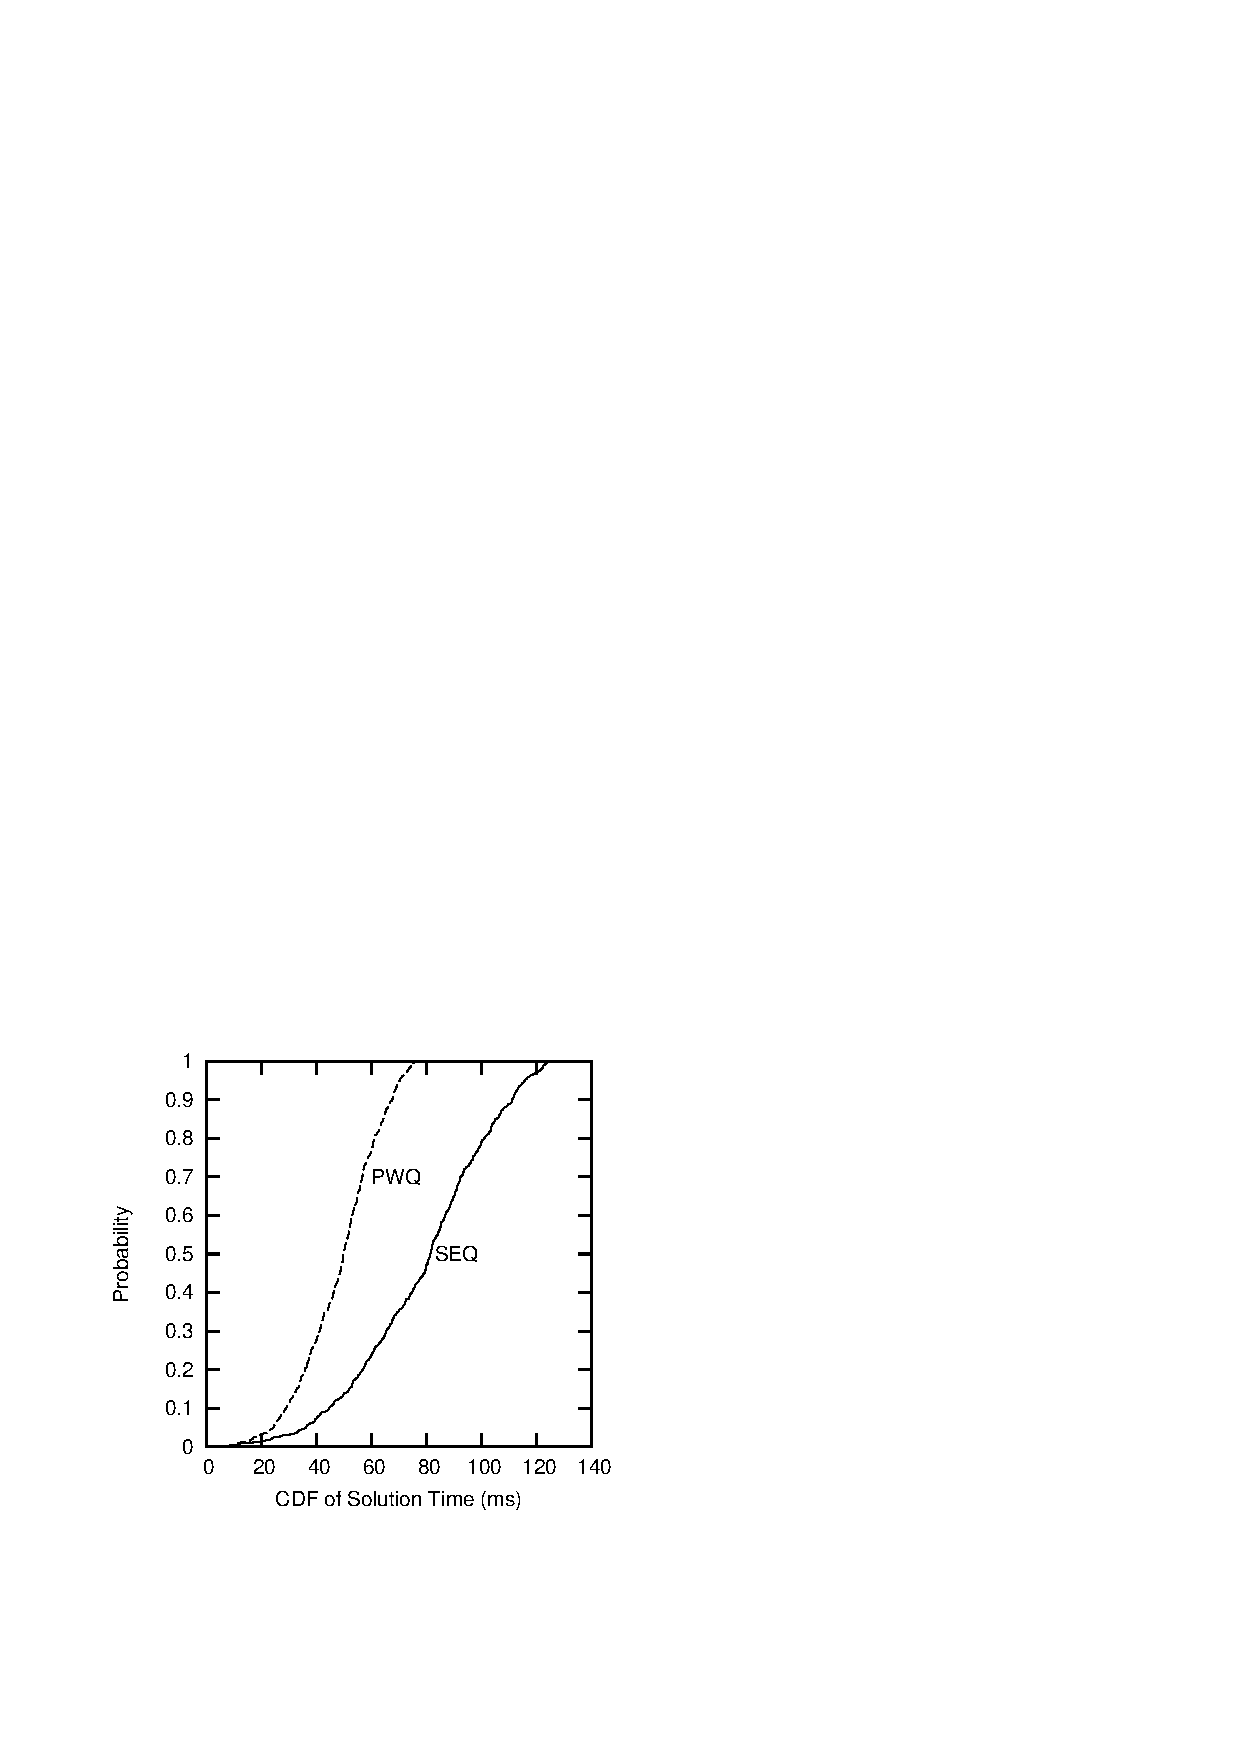
\includegraphics{SMPdesign/500-ms_seq_fg-cdf}}
\caption{CDF of Solution Times For SEQ and PWQ}
\label{fig:SMPdesign:CDF of Solution Times For SEQ and PWQ}
\end{figure}

병렬 work-queue solver 는
Listing~\ref{lst:SMPdesign:SEQ Pseudocode}
와~\ref{lst:SMPdesign:SEQ Helper Pseudocode} 에 보인 알고리즘의 간단한 병렬화
버전입니다.
\begin{fcvref}[ln:SMPdesign:SEQ Pseudocode]
Listing~\ref{lst:SMPdesign:SEQ Pseudocode} 의
\Clnref{ifge} 는 fetch-and-add 를 사용해야만 하며, 지역 변수 \co{vi} 는 다양한
쓰레드 사이에 공유되어야만 합니다.
\end{fcvref}
\begin{fcvref}[ln:SMPdesign:SEQ Helper Pseudocode:try]
Listing~\ref{lst:SMPdesign:SEQ Helper Pseudocode} 의
\clnref{chk:not:visited,mark:visited} 는 CAS 반복문으로 구성되어야만 하며, 이
반복문에서의 CAS 의 실패는 이 미로에서의 루프의 존재를 가리킵니다.
이 코드에서의 \clnrefrange{recordnext}{next:visited} 는 \co{->visited[]} 배열에
셀들을 기록하려는 동시적 시도들을 중재하기 위해 fetch-and-add 를 사용해야만
합니다.
\end{fcvref}

\iffalse

The parallel work-queue solver is a straightforward parallelization
of the algorithm shown in
Listings~\ref{lst:SMPdesign:SEQ Pseudocode} and~\ref{lst:SMPdesign:SEQ Helper Pseudocode}.
\begin{fcvref}[ln:SMPdesign:SEQ Pseudocode]
\Clnref{ifge} of Listing~\ref{lst:SMPdesign:SEQ Pseudocode} must use fetch-and-add,
and the local variable \co{vi} must be shared among the various threads.
\end{fcvref}
\begin{fcvref}[ln:SMPdesign:SEQ Helper Pseudocode:try]
\Clnref{chk:not:visited,mark:visited} of Listing~\ref{lst:SMPdesign:SEQ Helper Pseudocode} must be
combined into a CAS loop, with CAS failure indicating a loop in the
maze.
\Clnrefrange{recordnext}{next:visited} of this listing must use
fetch-and-add to arbitrate concurrent
attempts to record cells in the \co{->visited[]} array.
\end{fcvref}

\fi

이 방법은 500개의 다른 500x500 크기의 무작위로 생성된 미로에 대한 이 두
알고리즘의 해결 시간의 누적분포함수 (CDF) 를 보이는
Figure~\ref{fig:SMPdesign:CDF of Solution Times For SEQ and PWQ} 에 보인 것처럼
2.53\,GHz 에서 동작하는 듀얼 CPU Lenovo W500 에서 상당한 성능향상을 보입니다.
이 CDF 의 x 축으로의 상당한 겹치는 부분은
Section~\ref{sec:SMPdesign:Performance Comparison I} 에서 다뤄질 겁니다.

흥미롭게도, 순차적인 해결책-경로 탐색은 병렬 알고리즘에서도 바뀌지 않았습니다.
하지만, 이는 이 병렬 알고리즘의 상당한 약점을 덮지 못합니다:
항상 최대 하나의 쓰레드만이 이 해결책 경로에서 성과를 낼 수 있습니다.
이 약점은 다음 섹션에서 다룹니다.

\iffalse

This approach does provide significant speedups on a dual-CPU
Lenovo W500 running at 2.53\,GHz, as shown in
Figure~\ref{fig:SMPdesign:CDF of Solution Times For SEQ and PWQ},
which shows the cumulative distribution functions (CDFs) for the solution
times of the two algorithms, based on the solution of 500 different square
500-by-500 randomly generated mazes.
The substantial overlap
of the projection of the CDFs onto the x-axis will be addressed in
Section~\ref{sec:SMPdesign:Performance Comparison I}.

Interestingly enough, the sequential solution-path tracking works unchanged
for the parallel algorithm.
However, this uncovers a significant weakness in the parallel algorithm:
At most one thread may be making progress along the solution path at
any given time.
This weakness is addressed in the next section.

\fi

\subsection{Alternative Parallel Maze Solver}
\label{sec:SMPdesign:Alternative Parallel Maze Solver}

젊은 미로 해결기는 종종 양 끝에서 시작될 것을 요구받고, 이 조언은 자동화된 미로
탐색의 맥락에서 최근 더욱 반복되었습니다~\cite{UMD:CMSC433maze}.
이 조언은 운영체제 커널~\cite{Beck85,Inman85} 와
어플리케이션~\cite{DavidAPatterson2010TroubleMulticore} 모두를 위한 병렬
프로그래밍의 맥락에서 강력한 병렬화 전략인 파티셔닝이 됩니다.
이 섹션은 해결 경로의 반대 끝단에서 시작하는 두개의 자식 쓰레드를 사용해 이
전략을 적용해 보고, 성능과 확장성 결과에 대해 짧게 알아봅니다.

\iffalse

Youthful maze solvers are often urged to start at both ends, and
this advice has been repeated more recently in the context of automated
maze solving~\cite{UMD:CMSC433maze}.
This advice amounts to partitioning, which has been a powerful
parallelization strategy
in the context of parallel programming for both operating-system
kernels~\cite{Beck85,Inman85} and
applications~\cite{DavidAPatterson2010TroubleMulticore}.
This section applies this strategy, using two child threads that start
at opposite ends of the solution path, and takes a brief look at the
performance and scalability consequences.

\fi

\begin{listing}[tbp]
\begin{fcvlabel}[ln:SMPdesign:Partitioned Parallel Solver Pseudocode]
\begin{VerbatimL}[commandchars=\\\@\$]
int maze_solve_child(maze *mp, cell *visited, cell sc)	\lnlbl@b$
{
	cell c;
	cell n;
	int vi = 0;

	myvisited = visited; myvi = &vi;		\lnlbl@store:ptr$
	c = visited[vi];				\lnlbl@retrieve$
	do {
		while (!maze_find_any_next_cell(mp, c, &n)) {
			if (visited[++vi].row < 0)
				return 0;
			if (READ_ONCE(mp->done))	\lnlbl@chk:done1$
				return 1;
			c = visited[vi];
		}
		do {
			if (READ_ONCE(mp->done))	\lnlbl@chk:done2$
				return 1;
			c = n;
		} while (maze_find_any_next_cell(mp, c, &n));
		c = visited[vi];
	} while (!READ_ONCE(mp->done));		\lnlbl@chk:done3$
	return 1;
}
\end{VerbatimL}
\end{fcvlabel}
\caption{Partitioned Parallel Solver Pseudocode}
\label{lst:SMPdesign:Partitioned Parallel Solver Pseudocode}
\end{listing}

\begin{fcvref}[ln:SMPdesign:Partitioned Parallel Solver Pseudocode]
Listing~\ref{lst:SMPdesign:Partitioned Parallel Solver Pseudocode}
(\path{maze_part.c}) 에 보인 파티셔닝 병렬 알괴즘 (PART) 은 SEQ 와 비슷하지만
몇가지 중요한 차이점이 있습니다.
첫째로, 각 자식 쓰레드는 각자의 \co{visited} 배열을 가지며, 이는 부모로부터
라인~\lnref{b} 에 보인 것처럼 전달받는데, 모두 [$-1$, $-1$] 으로 초기화 되야만
합니다.
라인~\lnref{store:ptr} 은 이 배열로의 포인터를 쓰레드별 변수 \co{myvisited} 에
도움 주는 함수들에 의한 접근을 허용하기 위해 저장하며, 비슷하게 지역별 방문
인덱스로의 포인터도 저장합니다.
둘째로, 부모는 각 자식들 대신 첫번째 셀을 방문하는데, 이 자식들은 이를
라인~\lnref{retrieve} 에서 얻습니다.
셋째로, 이 미로는 한 자식이 다른 자식이 방문한 셀을 찾는 순간 해결됩니다.
넷째, 각 자식은 따라서 라인~\lnref{chk:done1}, \lnref{chk:done2},
그리고~\lnref{chk:done3} 에 보인 것처럼 주기적으로 \co{->done} 필드를 체크해야
합니다.
\co{READ_ONCE()} 기능은 뒤따르는 로드들을 합치거나 이 값을 다시 로드할 수 있는
모든 컴파일러 최적화를 불능화 시켜야 합니다.
C++1x volatile relaxed load 로도 충분할 겁니다~\cite{RichardSmith2019N4800}.
마지막으로, \co{maze_find_any_next_cell()} 함수는 한 셀을 방문되었다고 표시하기
위해 compare-and-swap 을 사용해야만 합니다만, 쓰레드 생성과 대기에 의해 제공된
것들 외에는 순서보장이 필요치 않습니다.
\end{fcvref}

\iffalse

\begin{fcvref}[ln:SMPdesign:Partitioned Parallel Solver Pseudocode]
The partitioned parallel algorithm (PART), shown in
Listing~\ref{lst:SMPdesign:Partitioned Parallel Solver Pseudocode}
(\path{maze_part.c}),
is similar to SEQ, but has a few important differences.
First, each child thread has its own \co{visited} array, passed in by
the parent as shown on line~\lnref{b},
which must be initialized to all [$-1$, $-1$].
Line~\lnref{store:ptr} stores a pointer to this array into the per-thread variable
\co{myvisited} to allow access by helper functions, and similarly stores
a pointer to the local visit index.
Second, the parent visits the first cell on each child's behalf,
which the child retrieves on line~\lnref{retrieve}.
Third, the maze is solved as soon as one child locates a cell that has
been visited by the other child.
When \co{maze_try_visit_cell()} detects this,
it sets a \co{->done} field in the maze structure.
Fourth, each child must therefore periodically check the \co{->done}
field, as shown on lines~\lnref{chk:done1}, \lnref{chk:done2}, and~\lnref{chk:done3}.
The \co{READ_ONCE()} primitive must disable any compiler
optimizations that might combine consecutive loads or that
might reload the value.
A C++1x volatile relaxed load suffices~\cite{RichardSmith2019N4800}.
Finally, the \co{maze_find_any_next_cell()} function must use
compare-and-swap to mark a cell as visited, however
no constraints on ordering are required beyond those provided by
thread creation and join.
\end{fcvref}

\fi

\begin{listing}[tbp]
\begin{fcvlabel}[ln:SMPdesign:Partitioned Parallel Helper Pseudocode]
\begin{VerbatimL}[commandchars=\\\@\$]
int maze_try_visit_cell(struct maze *mp, int c, int t,
                        int *n, int d)
{
	cell_t t;
	cell_t *tp;
	int vi;

	if (!maze_cells_connected(mp, c, t))		\lnlbl@chk:conn:b$
		return 0;				\lnlbl@chk:conn:e$
	tp = celladdr(mp, t);
	do {						\lnlbl@loop:b$
		t = READ_ONCE(*tp);
		if (t & VISITED) {			\lnlbl@chk:visited$
			if ((t & TID) != mytid)		\lnlbl@chk:other$
				mp->done = 1;		\lnlbl@located$
			return 0;			\lnlbl@ret:fail$
		}
	} while (!CAS(tp, t, t | VISITED | myid | d));	\lnlbl@loop:e$
	*n = t;						\lnlbl@update:new$
	vi = (*myvi)++;					\lnlbl@update:visited:b$
	myvisited[vi] = t;				\lnlbl@update:visited:e$
	return 1;					\lnlbl@ret:success$
}
\end{VerbatimL}
\end{fcvlabel}
\caption{Partitioned Parallel Helper Pseudocode}
\label{lst:SMPdesign:Partitioned Parallel Helper Pseudocode}
\end{listing}

\begin{fcvref}[ln:SMPdesign:Partitioned Parallel Helper Pseudocode]
\co{maze_find_any_next_cell()} 의 수도코드는
Listing~\ref{lst:SMPdesign:SEQ Helper Pseudocode} 에 보인 것과 동일합니다만,
\co{maze_try_visit_cell()} 의 수도코드는 다르며,
Listing~\ref{lst:SMPdesign:Partitioned Parallel Helper Pseudocode} 에 보이고
있습니다.
\Clnrefrange{chk:conn:b}{chk:conn:e} 는 이 셀들이 연결되어 있는지 검사하고,
그렇지 않다면 실패를 리턴합니다.
\Clnrefrange{loop:b}{loop:e} 의 루프는 이 새 셀을 방문되었다고 표시합니다.
라인~\lnref{chk:visited} 는 이게 이미 방문되었는지 검사하고, 그 경우에는
라인~\lnref{ret:fail} 에서 실패를 리턴합니다만, 라인~\lnref{chk:other} 난
우리가 다른 쓰레드를 만났는지 검사한 후이며, 그 경우에는 라인~\lnref{located}
에서 해결이 찾아졌다고 알립니다.
라인~\lnref{update:new} 는 새로운 셀로 업데이트를 하며,
라인~\lnref{update:visited:b} 와~\lnref{update:visited:e} 는 이 쓰레드의 방문된
셀들 배열을 업데이트 하고 라인~\lnref{ret:success} 에서 성공을 리턴합니다.
\end{fcvref}

\iffalse

\begin{fcvref}[ln:SMPdesign:Partitioned Parallel Helper Pseudocode]
The pseudocode for \co{maze_find_any_next_cell()} is identical to that shown in
Listing~\ref{lst:SMPdesign:SEQ Helper Pseudocode},
but the pseudocode for \co{maze_try_visit_cell()} differs, and
is shown in
Listing~\ref{lst:SMPdesign:Partitioned Parallel Helper Pseudocode}.
\Clnrefrange{chk:conn:b}{chk:conn:e}
check to see if the cells are connected, returning failure
if not.
The loop spanning \clnrefrange{loop:b}{loop:e} attempts to mark
the new cell visited.
Line~\lnref{chk:visited} checks to see if it has already been visited, in which case
line~\lnref{ret:fail} returns failure, but only after line~\lnref{chk:other}
checks to see if
we have encountered the other thread, in which case line~\lnref{located} indicates
that the solution has been located.
Line~\lnref{update:new} updates to the new cell,
lines~\lnref{update:visited:b} and~\lnref{update:visited:e} update this thread's visited
array, and line~\lnref{ret:success} returns success.
\end{fcvref}

\fi

\begin{figure}[tb]
\centering
\resizebox{2.2in}{!}{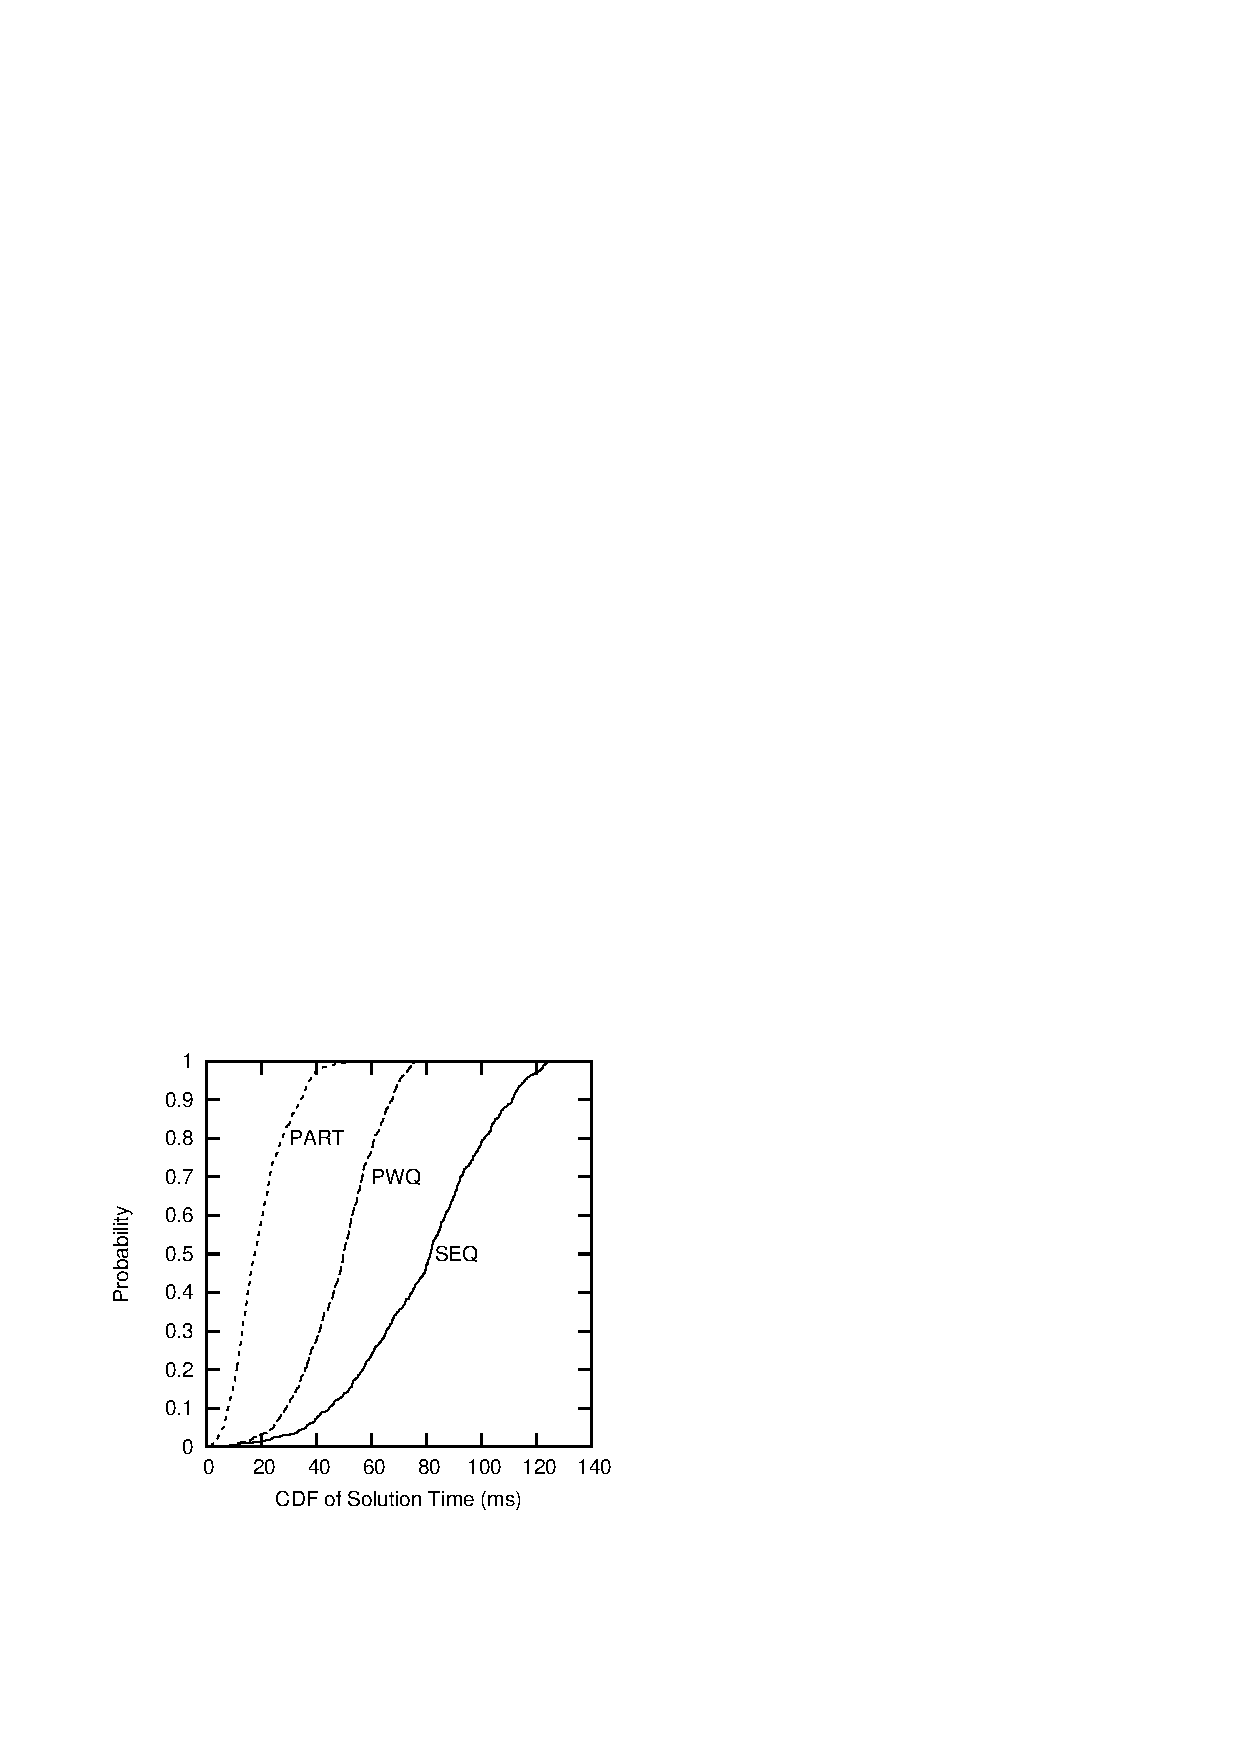
\includegraphics{SMPdesign/500-ms_seq_fg_part-cdf}}
\caption{CDF of Solution Times For SEQ, PWQ, and PART}
\label{fig:SMPdesign:CDF of Solution Times For SEQ, PWQ, and PART}
\end{figure}

성능 테스트는 놀라운 결과를 드러냈는데,
Figure~\ref{fig:SMPdesign:CDF of Solution Times For SEQ, PWQ, and PART} 에 보여
있습니다.
PART 의 중간 해결 시간 (17 밀리세컨드) 는 SEQ 의 것 (79 밀리세컨드) 보다 두개의
쓰레드만을 사용하고 있음에도 네배가 넘게 빨랐습니다.
다음 섹션에서 이 결과를 분석해 봅니다.

\iffalse

Performance testing revealed a surprising anomaly, shown in
Figure~\ref{fig:SMPdesign:CDF of Solution Times For SEQ, PWQ, and PART}.
The median solution time for PART (17 milliseconds)
is more than four times faster than that of SEQ (79 milliseconds),
despite running on only two threads.
The next section analyzes this anomaly.

\fi

\subsection{Performance Comparison I}
\label{sec:SMPdesign:Performance Comparison I}

\begin{figure}[tb]
\centering
\resizebox{2.2in}{!}{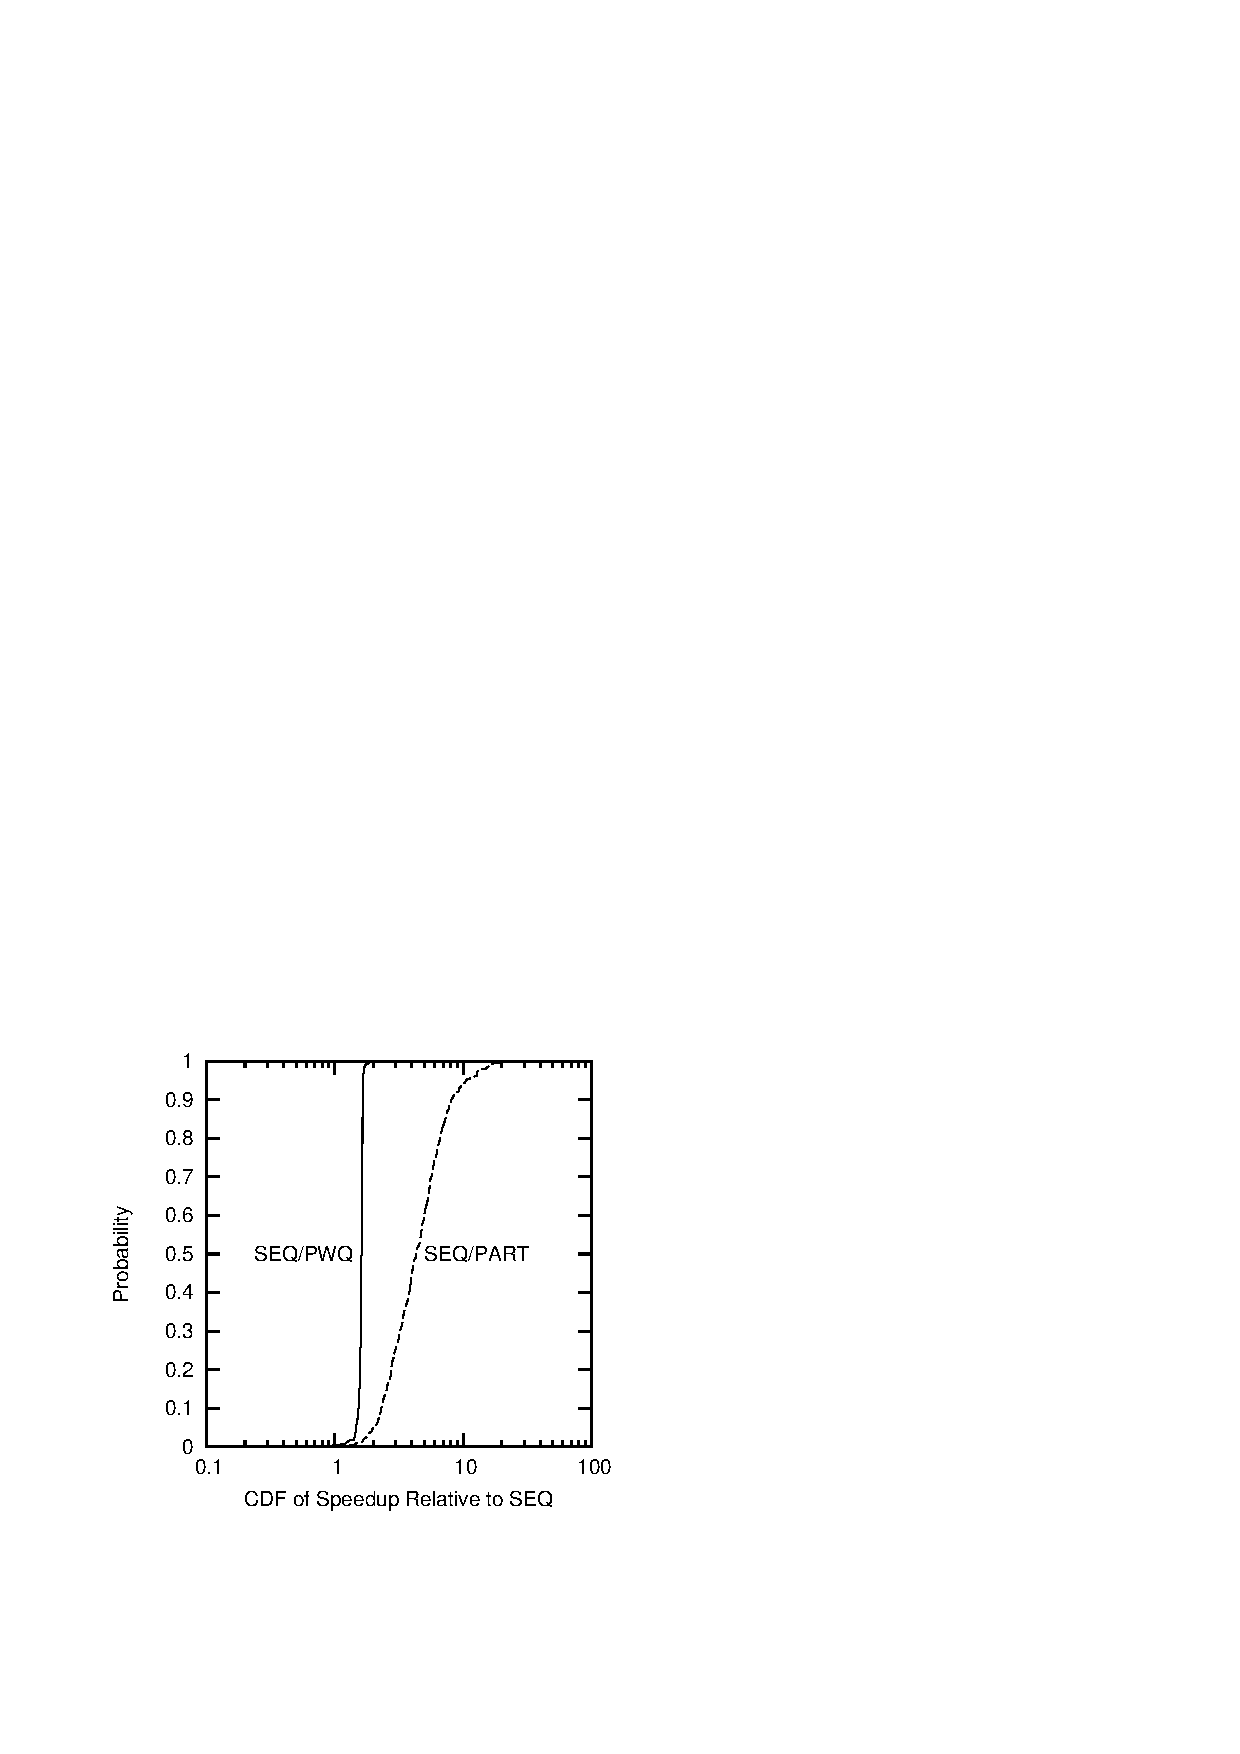
\includegraphics{SMPdesign/500-ms_seqVfg_part-cdf}}
\caption{CDF of SEQ/PWQ and SEQ/PART Solution-Time Ratios}
\label{fig:SMPdesign:CDF of SEQ/PWQ and SEQ/PART Solution-Time Ratios}
\end{figure}

예상 외의 성능 결과에 대해 해야할 첫번째 반응은 버그 검사입니다.
이 알고리즘은 실제로 유효한 미로 해법을 찾아냈지만,
Figure~\ref{fig:SMPdesign:CDF of Solution Times For SEQ, PWQ, and PART}
의 CDF 그림은 비종속적 데이터 포인트들을 가정합니다.
이건 그 경우가 아닙니다:  이 성능 테스트는 무작위로 미로를 만들어내고, 모든
미로 해법기를 해당 미로에 대해 동작시킵니다.
따라서
Figure~\ref{fig:SMPdesign:CDF of SEQ/PWQ and SEQ/PART Solution-Time Ratios}
에 보인 것처럼 각각의 생성된 미로에 대한 해결책 시간의 비율을 CDF 로 그리는게
합리적이며, CDF 들의 겹침을 크게 줄여줍니다.
이 그림은 일부 미로에 대해선, PART 가 SEQ 보다 \emph{40} 배가 넘게 빠름을
보입니다.
대조적으로, PWQ 는 SEQ 보다 두배 이상 빠르지 않습니다.
두 쓰레드를 사용하고 40배의 속도향상을 이룬것에 대해선 설명이 필요합니다.
어쨌건, 이건 그냥 파티셔닝 가능성은 쓰레드를 추가하기만 한다는 것이 전체 계산
비용을 늘리지는 않음을 의미하는 당황스러울 정도의 병렬성이 아닙니다.
이건 그보다는 \emph{굴욕적인 병렬성} 입니다: 쓰레드를 추가하는 것이 전체 계산
비용을 줄여서 알고리즘의 초선형적 속도향상을 이뤘습니다.

\iffalse

The first reaction to a performance anomaly is to check for bugs.
Although the algorithms were in fact finding valid solutions, the
plot of CDFs in
Figure~\ref{fig:SMPdesign:CDF of Solution Times For SEQ, PWQ, and PART}
assumes independent data points.
This is not the case:  The performance tests randomly generate a maze,
and then run all solvers on that maze.
It therefore makes sense to plot the CDF of the ratios of
solution times for each generated maze,
as shown in
Figure~\ref{fig:SMPdesign:CDF of SEQ/PWQ and SEQ/PART Solution-Time Ratios},
greatly reducing the CDFs' overlap.
This plot reveals that for some mazes, PART
is more than \emph{forty} times faster than SEQ\@.
In contrast, PWQ is never more than about
two times faster than SEQ\@.
A forty-times speedup on two threads demands explanation.
After all, this is not merely embarrassingly parallel, where partitionability
means that adding threads does not increase the overall computational cost.
It is instead \emph{humiliatingly parallel}: Adding threads
significantly reduces the overall computational cost, resulting in
large algorithmic superlinear speedups.

\fi

\begin{figure}[tb]
\centering
\resizebox{1.4in}{!}{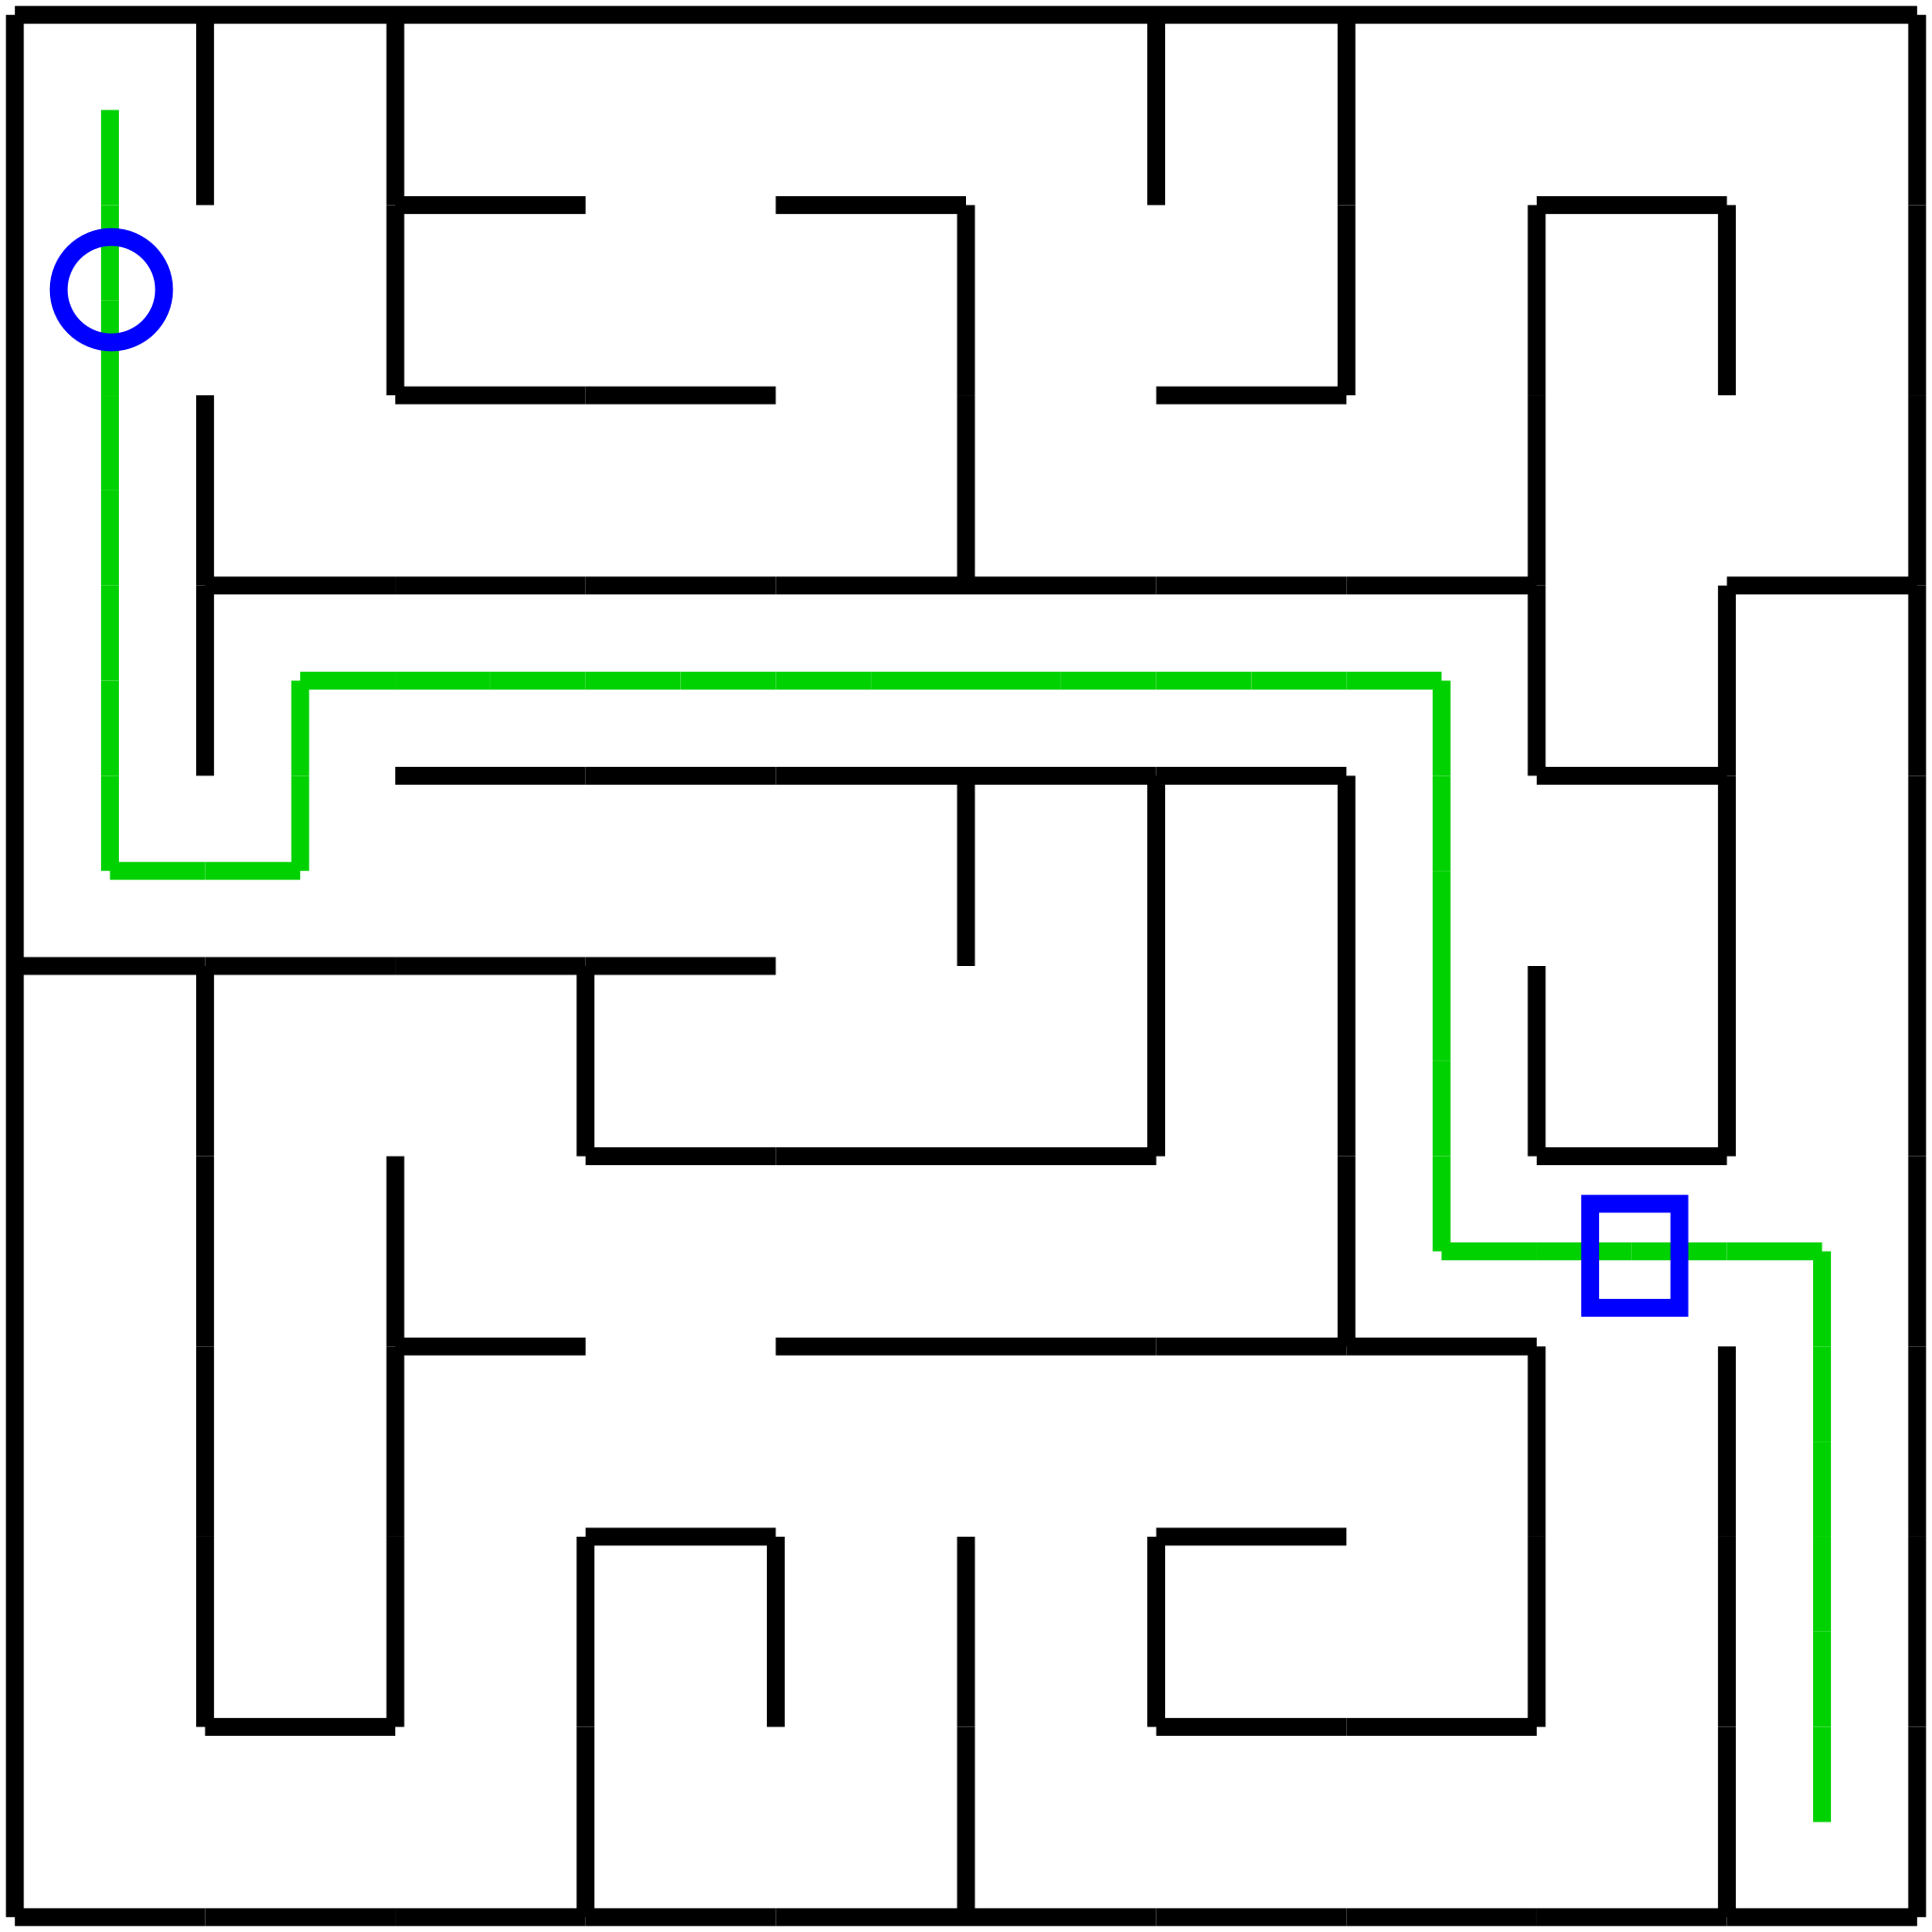
\includegraphics{SMPdesign/maze_in_way10a}}
\caption{Reason for Small Visit Percentages}
\label{fig:SMPdesign:Reason for Small Visit Percentages}
\end{figure}

\begin{figure}[tb]
\centering
\resizebox{2.2in}{!}{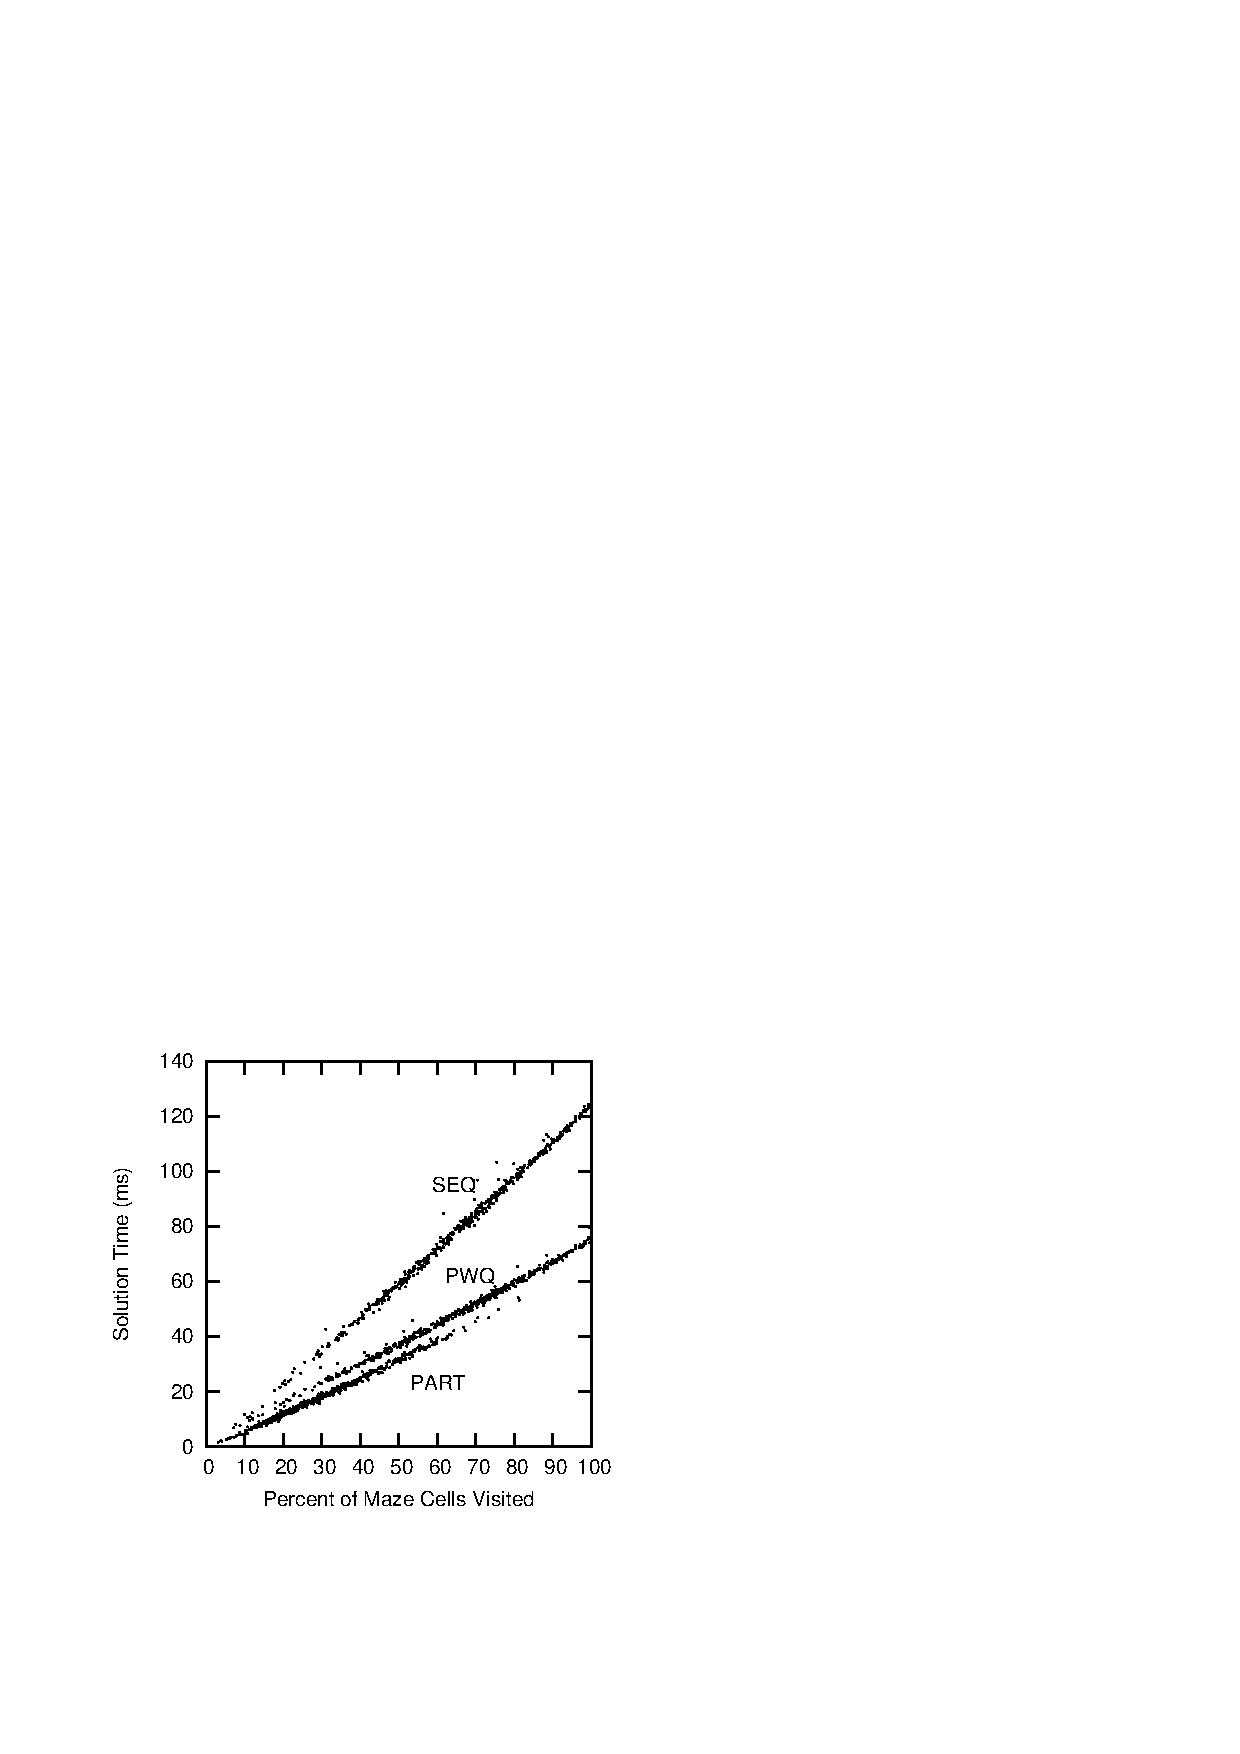
\includegraphics{SMPdesign/500-pctVms_seq_part-sct}}
\caption{Correlation Between Visit Percentage and Solution Time}
\label{fig:SMPdesign:Correlation Between Visit Percentage and Solution Time}
\end{figure}

계속된 조사는 PART 가 가끔은 미로의 셀들 중 2\,\% 미만의 것들만을 방문한 반면,
SEQ 와 PWQ 는 9\,\% 미만을 방문한 적이 없음을 드러냈습니다.
이 차이에 대한 이유는
Figure~\ref{fig:SMPdesign:Reason for Small Visit Percentages}
에 보여져 있습니다.
좌상단부터 해결책을 찾는 쓰레드가 원을 만나면, 다른 쓰레드는 미로의 우상단에
닿지 못합니다.
비슷하게, 이 다른 쓰레드가 네모를 만나면 첫번째 쓰레드는 미로의 좌하단에 닿지
못합니다.
따라서, PART 는 해법이 아닌 셀들의 작은 부분만을 방문하게 될 겁니다.
요약하자면, 이 초선형적 속도향상은 서로의 방향을 향하는 쓰레드들 때문입니다.
이는 각 쓰레드가 서로의 방향 \emph{바깥으로} 유지시키려 노력해왔던 병렬
프로그래밍에 대한 수십년의 경험에 상당히 대조적인 결과입니다.

Figure~\ref{fig:SMPdesign:Correlation Between Visit Percentage and Solution Time}
는 이 세개의 방법들의 해결책 탐색 시간과 방문된 셀들 사이의 강한 상관관계를
확인시켜 줍니다.
PART 의 그림의 비탈은 SEQ 의 것보다 작아서, PART 의 한쌍의 쓰레드는 미로의
주어진 부분을 SEQ 의 단일 쓰레드가 하는 것보다 빠르게 방문함을 보입니다.
PART 의 그림은 또한 작은 방문 퍼센티지로 기울어 있어서, PART 가 더 적은 전체
일을 하며, 따라서 굴욕적인 병렬성을 보였음을 확인시켜 줍니다.

\iffalse

Further investigation showed that
PART sometimes visited fewer than 2\,\% of the maze's cells,
while SEQ and PWQ never visited fewer than about 9\,\%.
The reason for this difference is shown by
Figure~\ref{fig:SMPdesign:Reason for Small Visit Percentages}.
If the thread traversing the solution from the upper left reaches
the circle, the other thread cannot reach
the upper-right portion of the maze.
Similarly, if the other thread reaches the square,
the first thread cannot reach the lower-left
portion of the maze.
Therefore, PART will likely visit a small fraction
of the non-solution-path cells.
In short, the superlinear speedups are due to threads getting in each
others' way.
This is a sharp contrast with decades of experience with
parallel programming, where workers have struggled
to keep threads \emph{out} of each others' way.

Figure~\ref{fig:SMPdesign:Correlation Between Visit Percentage and Solution Time}
confirms a strong correlation between cells visited and solution time
for all three methods.
The slope of PART's scatterplot is smaller than that of SEQ,
indicating that PART's pair of threads visits a given fraction
of the maze faster than can SEQ's single thread.
PART's scatterplot is also weighted toward small visit
percentages, confirming that PART does less total work, hence
the observed humiliating parallelism.

\fi

\begin{figure}[tb]
\centering
\resizebox{1.4in}{!}{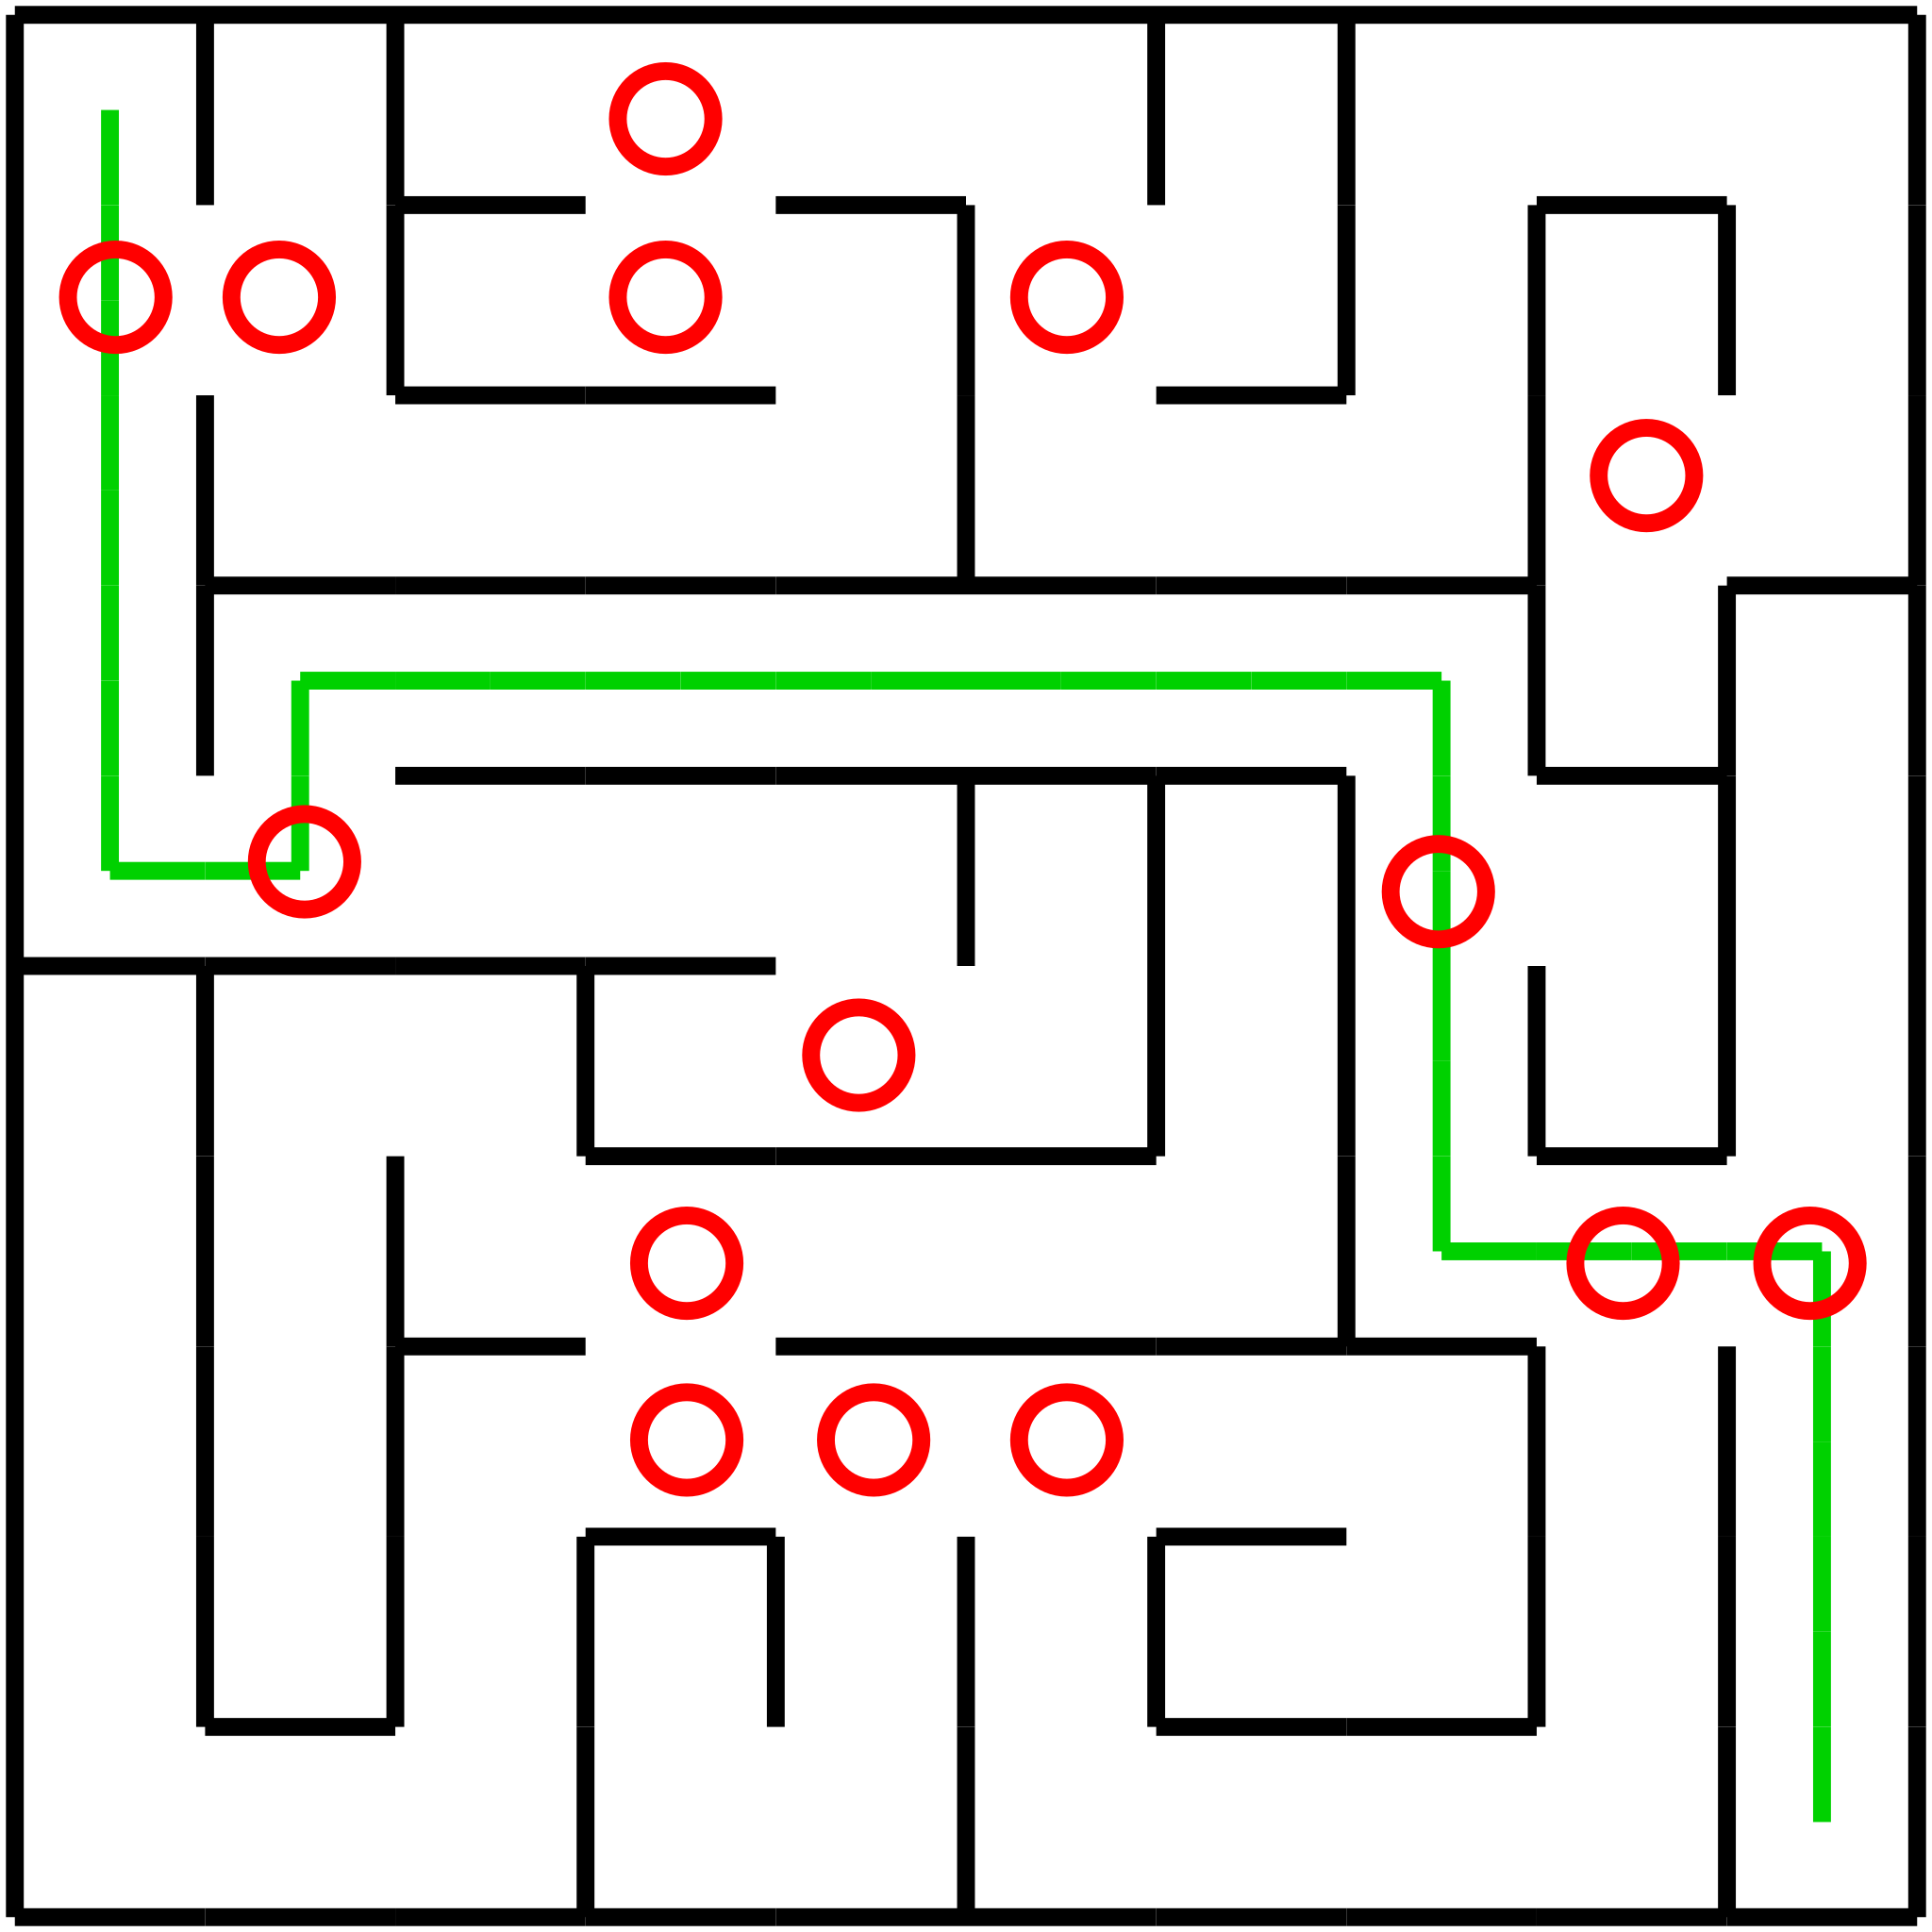
\includegraphics{SMPdesign/maze_PWQ_vs_PART}}
\caption{PWQ Potential Contention Points}
\label{fig:SMPdesign:PWQ Potential Contention Points}
\end{figure}

PWQ 에 의해 방문된 셀들의 부분은 SEQ 의 것과 비슷합니다.
또한, PWQ 의 해법 탐색 시간은 PART 의 그것보다 큰데, 비슷한 방문 비율에
대해서조차 그렇습니다.
이에 대한 이유가
Figure~\ref{fig:SMPdesign:PWQ Potential Contention Points} 에 그려져 있는데, 각
셀에 두개 이상의 이웃을 가진 빨간 원이 있습니다.
그런 각각의 셀은 PWQ 에서 컨텐션을 유발할 수 있는데, 한 쓰레드가 들어갈 수
있지만 두 쓰레드는 나올 수 없어서, 이 챕터의 앞부분에서 이야기 했듯 성능을
하락시키게 되기 때문입니다.
대조적으로, PART 는 그런 컨텐션을 한번만 일으키는데, 해결책이 찾아졌을
때입니다.
물론, SEQ 는 결코 컨텐션을 갖지 않습니다.

\iffalse

The fraction of cells visited by PWQ is similar to that of SEQ\@.
In addition, PWQ's solution time is greater than that of PART,
even for equal visit fractions.
The reason for this is shown in
Figure~\ref{fig:SMPdesign:PWQ Potential Contention Points}, which has a red
circle on each cell with more than two neighbors.
Each such cell can result in contention in PWQ, because
one thread can enter but two threads can exit, which hurts
performance, as noted earlier in this chapter.
In contrast, PART can incur such contention but once, namely
when the solution is located.
Of course, SEQ never contends.

\fi

\begin{figure}[tb]
\centering
\resizebox{2.2in}{!}{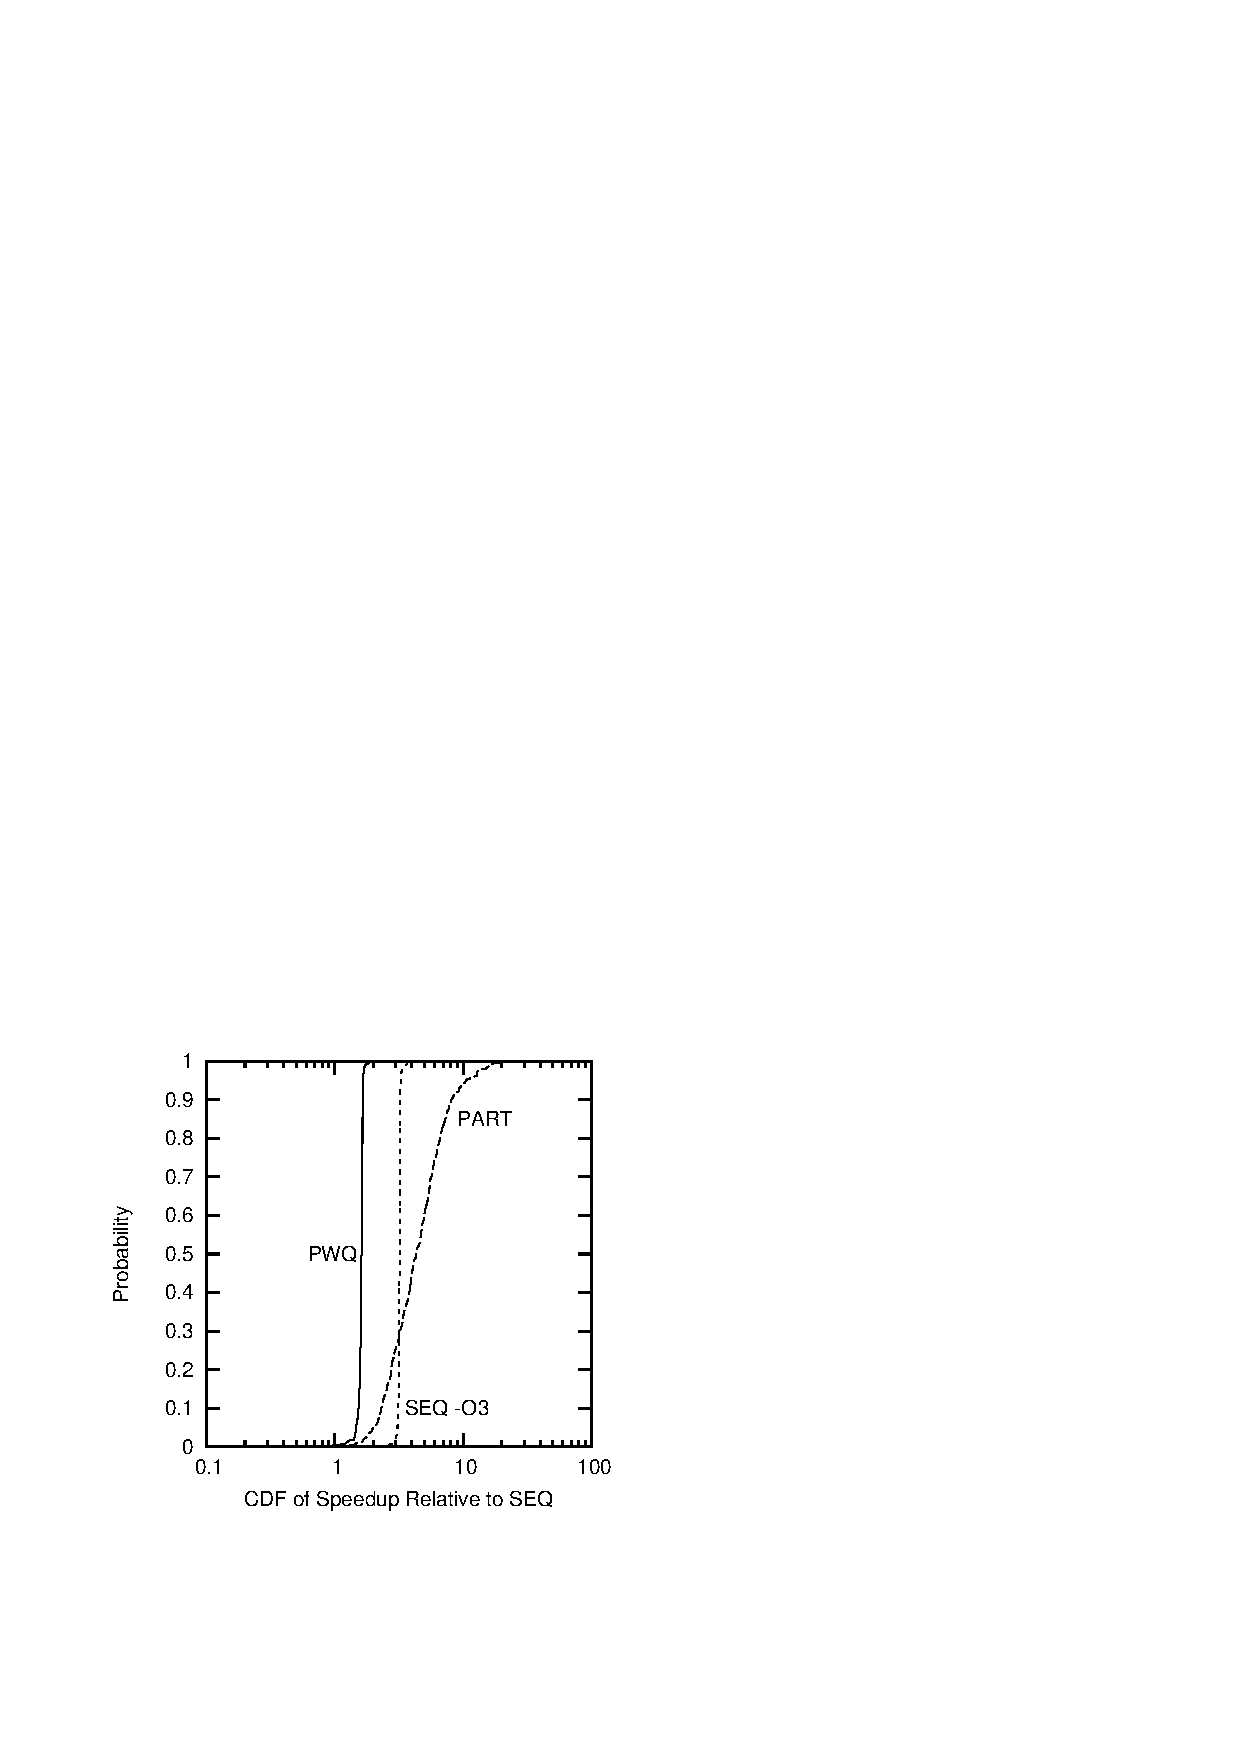
\includegraphics{SMPdesign/500-ms_seqVfg_part_seqO3-cdf}}
\caption{Effect of Compiler Optimization (-O3)}
\label{fig:SMPdesign:Effect of Compiler Optimization (-O3)}
\end{figure}

PART 의 속도 향상이 인상적이긴 하지만, 순차적 최적화를 무시해선 안됩니다.
Figure~\ref{fig:SMPdesign:Effect of Compiler Optimization (-O3)} 는 \co{-O3} 로
컴파일 되었을 때 SEQ 가 최적화 되지 않은 PWQ 보다 두배 가량 빨라서, 최적화 되지
않은 PART 에 근접함을 보입니다.
세 알고리즘을 모두 \co{-O3} 로 컴파일 했을 때의 결과는
Figure~\ref{fig:SMPdesign:CDF of SEQ/PWQ and SEQ/PART Solution-Time Ratios}
에 보인 것과 같이 (더 빨라졌긴 하지만) 비슷한 결과를 보이는데, PWQ 가 SEQ 에
비해 속도 향상은 거의 제공하지 않아, 암달의
법칙~\cite{GeneAmdahl1967AmdahlsLaw} 이 유지됨도 보입니다.
하지만, 목표가 최적화 자체가 아니라 최적화 되지 않은 SEQ 에 비해 두배의 성능을
달성하는 것이라면, 컴파일러 최적화는 상당히 매력적인 것입니다.

\iffalse

Although PART's speedup is impressive, we should not neglect sequential
optimizations.
Figure~\ref{fig:SMPdesign:Effect of Compiler Optimization (-O3)} shows that
SEQ, when compiled with \co{-O3}, is about twice as fast
as unoptimized PWQ, approaching the performance of unoptimized PART\@.
Compiling all three algorithms with \co{-O3} gives results similar to
(albeit faster than) those shown in
Figure~\ref{fig:SMPdesign:CDF of SEQ/PWQ and SEQ/PART Solution-Time Ratios},
except that PWQ provides almost no speedup compared
to SEQ, in keeping with Amdahl's Law~\cite{GeneAmdahl1967AmdahlsLaw}.
However, if the goal is to double performance compared to unoptimized
SEQ, as opposed to achieving optimality, compiler
optimizations are quite attractive.

\fi

캐쉬 정렬과 패딩은 거짓 공유를 줄임으로써 성능을 종종 향상시킵니다.
하지만, 이 미로 해법 탐색 알고리즘에서 미로 셀 배열을 정렬하고 패딩하는 것은
1000x1000 미로에 대해 최대 42\,\% 까지 성능을 \emph{떨어뜨립니다}.
캐쉬 지역성은 거짓 공유를 막는 것보다 더 중요하며, 특히 큰 미로에 대해선
그렇습니다.
더 작은 20-by-20 이나 50-by-50 미로들에 대해선 정렬과 패딩이 PART 의 경우 최대
40\,\% 성능 향상을 만들어냈습니다만, 그런 작은 크기에 대해서는 SEQ 가 어쨌건 더
나은데 PART 가 쓰레드생성과 정리에 드는 오버헤드를 감당할 중분한 시간이 없기
때문입니다.

요약하자면, 파티셔닝 된 병렬 미로 해법 탐색기는 알고리즘상의 초선형적
속도향상의 흥미로운 예입니다.
만약 ``알고리즘상의 초선형적 속도향상'' 이 인지부조화를 일으킨다면, 다음
섹션으로 넘어가시기 바랍니다.

\iffalse

Cache alignment and padding often improves performance by reducing
false sharing.
However, for these maze-solution algorithms, aligning and padding the
maze-cell array \emph{degrades} performance by up to 42\,\% for 1000x1000 mazes.
Cache locality is more important than avoiding
false sharing, especially for large mazes.
For smaller 20-by-20 or 50-by-50 mazes, aligning and padding can produce
up to a 40\,\% performance improvement for PART,
but for these small sizes, SEQ performs better anyway because there
is insufficient time for PART to make up for the overhead of
thread creation and destruction.

In short, the partitioned parallel maze solver is an interesting example
of an algorithmic superlinear speedup.
If ``algorithmic superlinear speedup'' causes cognitive dissonance,
please proceed to the next section.

\fi

\subsection{Alternative Sequential Maze Solver}
\label{sec:SMPdesign:Alternative Sequential Maze Solver}

\begin{figure}[tb]
\centering
\resizebox{2.2in}{!}{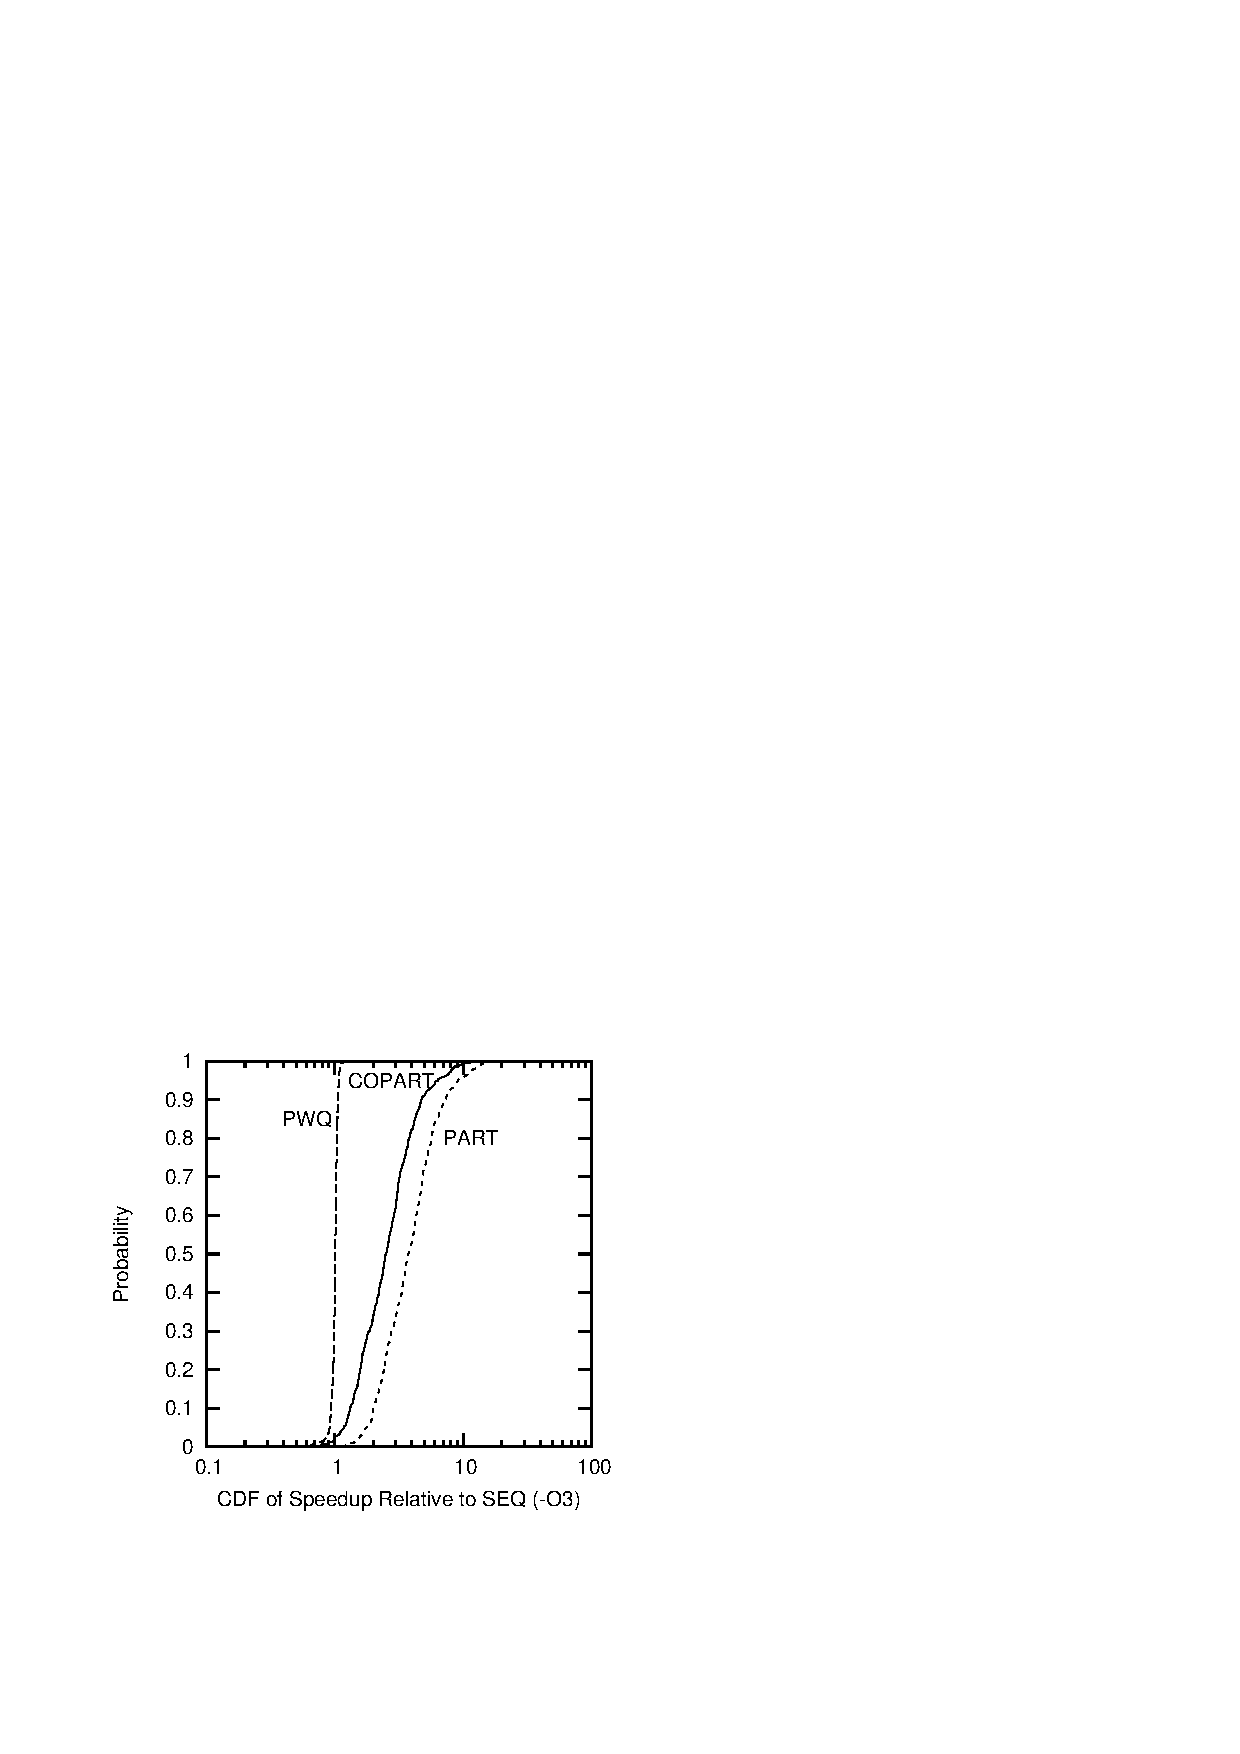
\includegraphics{SMPdesign/500-ms_seqO3V2seqO3_fgO3_partO3-cdf}}
\caption{Partitioned Coroutines}
\label{fig:SMPdesign:Partitioned Coroutines}
\end{figure}

알고리즘상의 초선형적 속도향상의 존재는 예를 들면
Listing~\ref{lst:SMPdesign:Partitioned Parallel Solver Pseudocode} 의 메인
do-while 루프를 통과하는 각 패스에서 쓰레드간에 일일이 컨텍스트 스위칭 (context
switching) 을 하는 식의, 코루틴을 통한 병렬성을 시뮬레이션 해볼 것을
제안합니다.
이 컨텍스트 스위칭은 이 컨텍스트가 변수 \co{c} 와 \co{vi} 만으로 구성되어 있기
때문에 간단합니다: 이 효과를 이룰 수 있는 많은 방법들 가운데, 이는 컨텍스트
스위치 오버헤드와 방문 퍼센티지 사이의 좋은 트레이드오프입니다.
Figure~\ref{fig:SMPdesign:Partitioned Coroutines}
에서 볼 수 있듯, 이 코루틴 알고리즘 (COPART) 은 상당히 효과적으로, 단일
쓰레드로 두개 쓰레드를 사용하는 PART 의 30\,\% 정도 성능이 됩니다
(\path{maze_2seq.c}).

\iffalse

The presence of algorithmic superlinear speedups suggests simulating
parallelism via co-routines, for example, manually switching context
between threads on each pass through the main do-while loop in
Listing~\ref{lst:SMPdesign:Partitioned Parallel Solver Pseudocode}.
This context switching is straightforward because the context
consists only of the variables \co{c} and \co{vi}: Of the numerous
ways to achieve the effect, this is a good tradeoff between
context-switch overhead and visit percentage.
As can be seen in
Figure~\ref{fig:SMPdesign:Partitioned Coroutines},
this coroutine algorithm (COPART) is quite effective, with the performance
on one thread being within about 30\,\% of PART on two threads
(\path{maze_2seq.c}).

\fi

\subsection{Performance Comparison II}
\label{sec:SMPdesign:Performance Comparison II}

\begin{figure}[tb]
\centering
\resizebox{2.2in}{!}{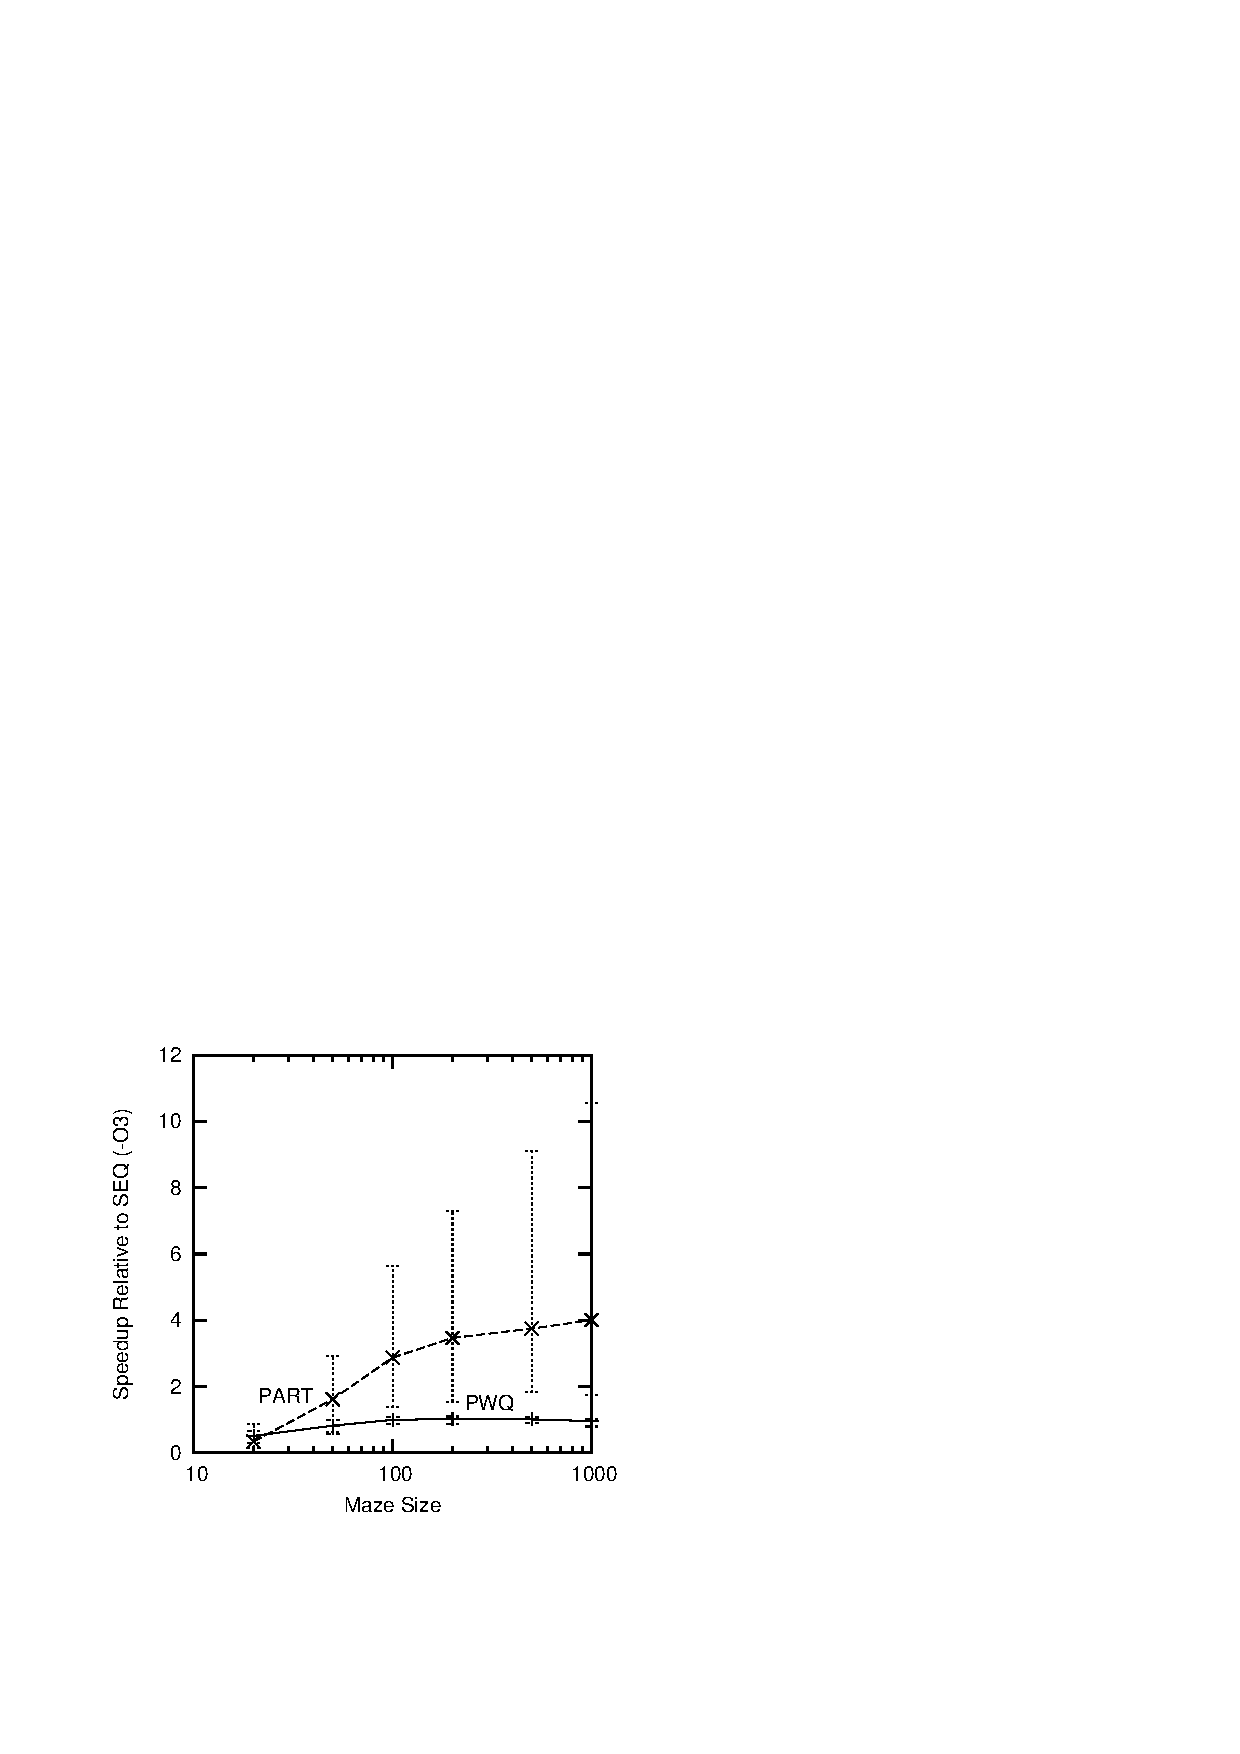
\includegraphics{SMPdesign/500-ms_seqO3VfgO3_partO3-median}}
\caption{Varying Maze Size vs. SEQ}
\label{fig:SMPdesign:Varying Maze Size vs. SEQ}
\end{figure}

\begin{figure}[tb]
\centering
\resizebox{2.2in}{!}{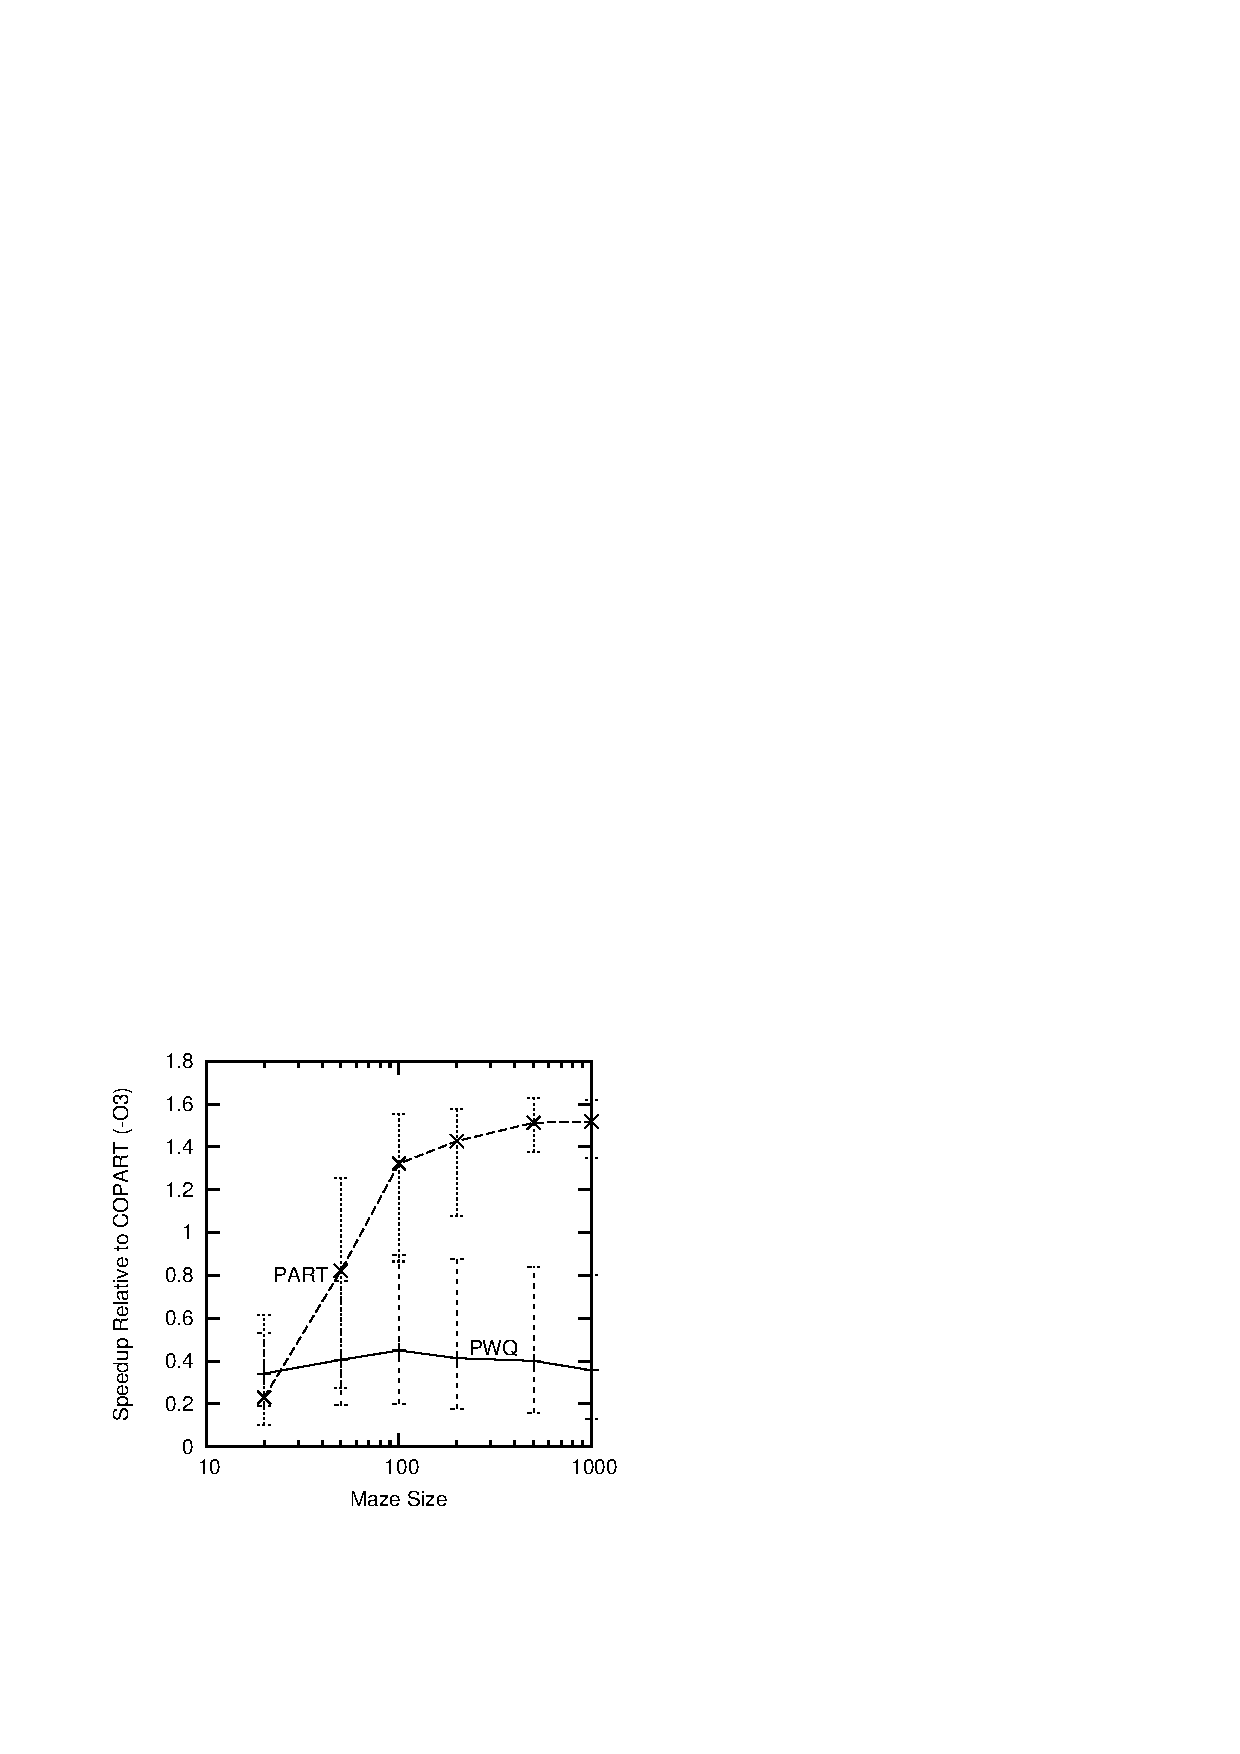
\includegraphics{SMPdesign/500-ms_2seqO3VfgO3_partO3-median}}
\caption{Varying Maze Size vs. COPART}
\label{fig:SMPdesign:Varying Maze Size vs. COPART}
\end{figure}

Figure~\ref{fig:SMPdesign:Varying Maze Size vs. SEQ}
와~\ref{fig:SMPdesign:Varying Maze Size vs. COPART}
는 당야한 미로 크기에 대해 이 효과를 보이는데, 두개의 쓰레드를 사용해 동작하는
PWQ 와 PART 를 SEQ 또는 COPART 에 대해 각각 비교하는데,
90\=/percent\-/confidence 에러바도 보입니다.
PART 는 100-by-100 과 그보다 큰 미로에 있어선 SEQ 에 비교해 초선형적인, 그리고
COPART 에 대해선 약간의 확장성을 보입니다.
대략 200-by-200 미로 크기부터는 전력 소모는 대략적으로 높은 주파수에서는
주파수의 제곱에 비례하여~\cite{TrevorMudge2000Power} 두 쓰레드에서의 1.4x
확장은 똑같은 해법 탐색 시간에서의 단일 쓰레드와 같은 전력을 소모하므로
200-by-200 미로 크기부터는 PART 는 COPART 의 이론적 에너지 효율성 손익분기를
넘어섭니다.
대조적으로, PWQ 는 SEQ 와 COPART 모두에 대해 최적화가 되지 않은 상태가 아니고는
낮은 확장성을 보입니다: Figure~\ref{fig:SMPdesign:Varying Maze Size vs. SEQ} 
와~\ref{fig:SMPdesign:Varying Maze Size vs. COPART}
는 \co{-O3} 를 사용해 만들어졌습니다.

\iffalse

Figures~\ref{fig:SMPdesign:Varying Maze Size vs. SEQ}
and~\ref{fig:SMPdesign:Varying Maze Size vs. COPART}
show the effects of varying maze size, comparing both PWQ and PART
running on two threads
against either SEQ or COPART, respectively, with 90\=/percent\-/confidence
error bars.
PART shows superlinear scalability against SEQ and modest scalability
against COPART for 100-by-100 and larger mazes.
PART exceeds theoretical energy-efficiency breakeven against COPART at roughly
the 200-by-200 maze size, given that power consumption rises as roughly
the square of the frequency for high frequencies~\cite{TrevorMudge2000Power},
so that 1.4x scaling on two threads consumes the same energy
as a single thread at equal solution speeds.
In contrast, PWQ shows poor scalability against both SEQ and COPART
unless unoptimized: Figures~\ref{fig:SMPdesign:Varying Maze Size vs. SEQ} 
and~\ref{fig:SMPdesign:Varying Maze Size vs. COPART}
were generated using \co{-O3}.

\fi

\begin{figure}[tb]
\centering
\resizebox{2.2in}{!}{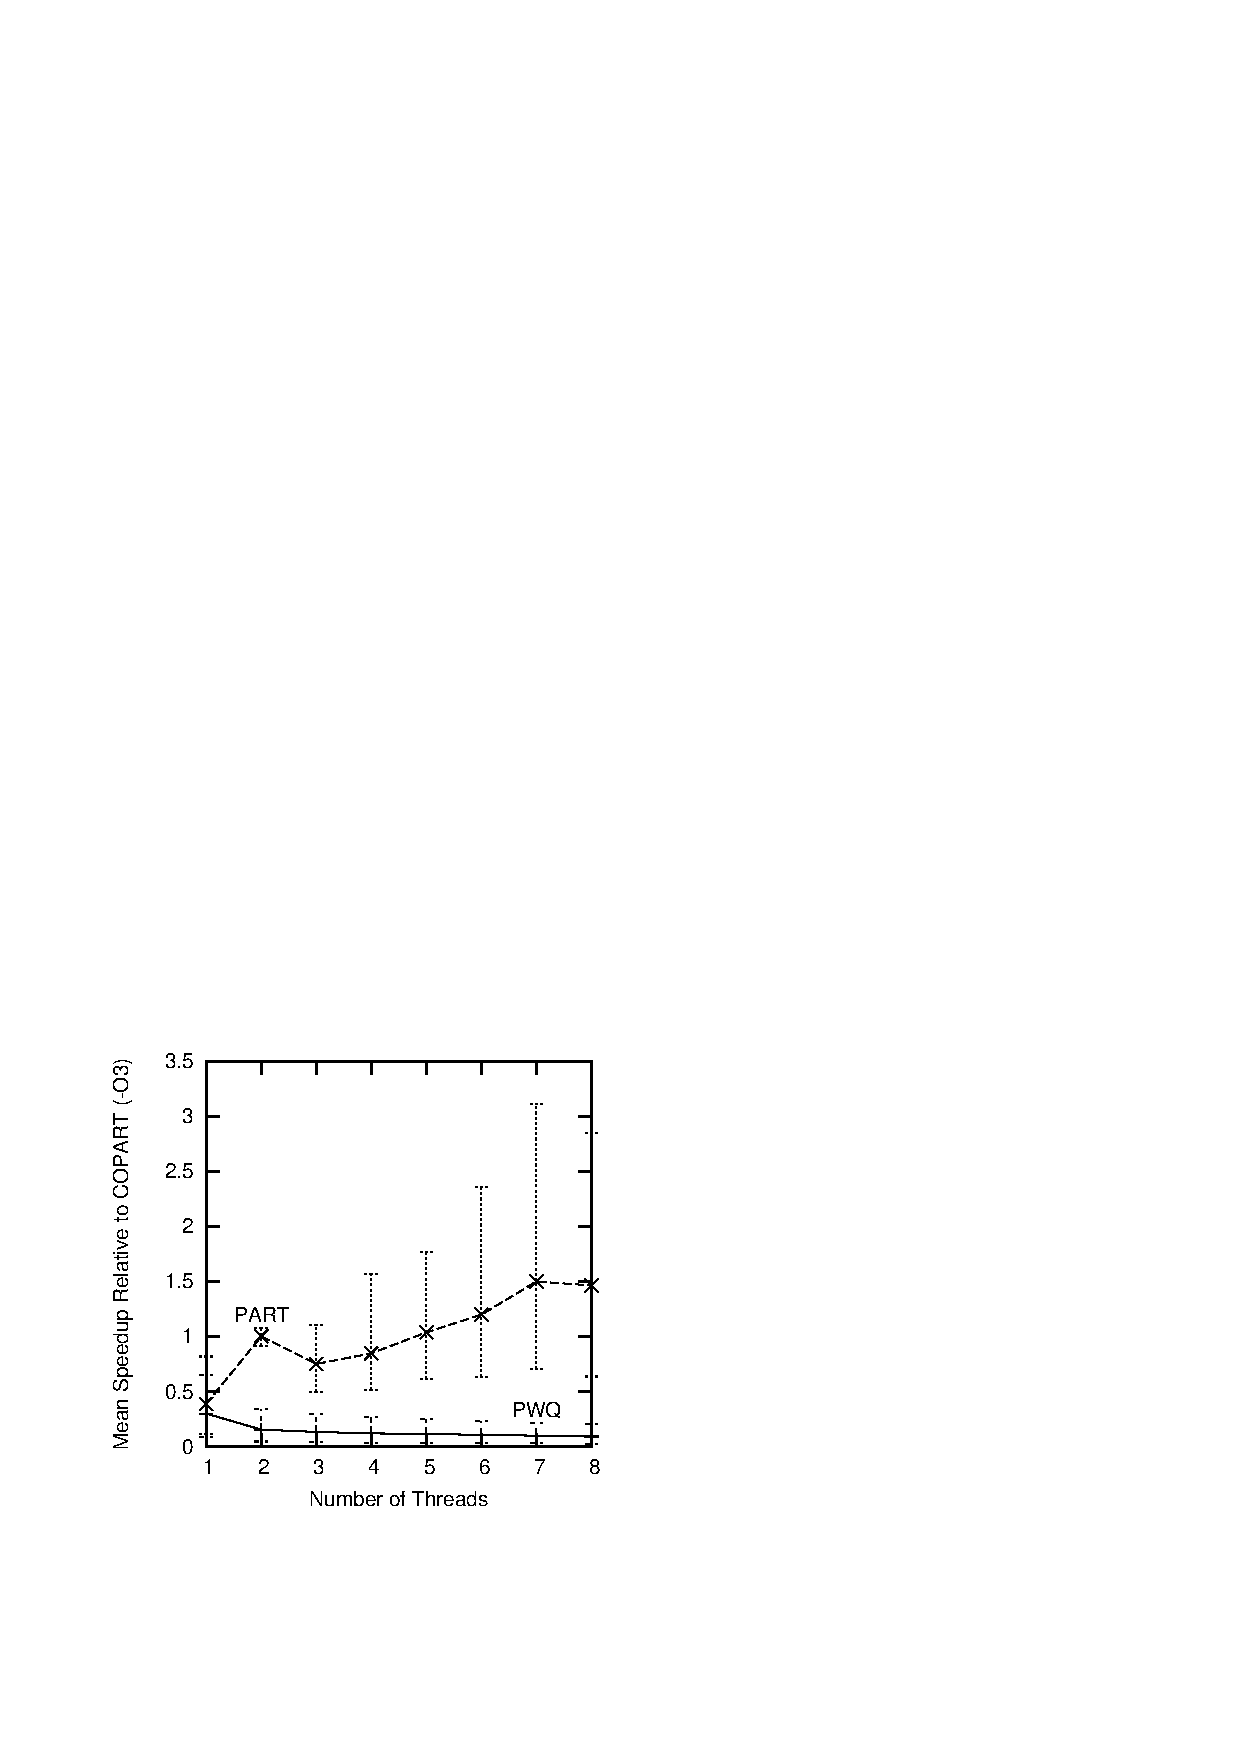
\includegraphics{SMPdesign/1000-ms_2seqO3VfgO3_partO3-mean}}
\caption{Mean Speedup vs. Number of Threads, 1000x1000 Maze}
\label{fig:SMPdesign:Mean Speedup vs. Number of Threads, 1000x1000 Maze}
\end{figure}

Figure~\ref{fig:SMPdesign:Mean Speedup vs. Number of Threads, 1000x1000 Maze}
는 PWQ 와 PART 의 성능을 COPART 에 상대적으로 보입니다.
두개가 넘는 쓰레드로 돌아가는 PART 를 위해선, 추가된 쓰레드는 시작과 끝 셀을
연결하는 대각선상에서 똑같이 나뉘어진 위치에서 시작되었습니다.
두개 이상의 쓰레드를 사용해 동작하는 PART 의 조기 종료를 알아내기 위해 단순화된
연결 상태 라우팅~\cite{BERT-87} 이 사용되었습니다 (한 쓰레드가 시작과 끝과 모두
연결되었을 때 해결책이 찾아진 것으로 취급됩니다).
PWQ 는 무척 처참한 성능을 보입니다만, PART 는 두개 쓰레드에서 손익분기를 치고
5개 쓰레드에서도 그런데, 다섯개 쓰레드 이후부턴 약간의 속도향상만 달성합니다.
이론적 전력 효율성 손익분기는 7개와 8개 쓰레드에 대해선
90\=/percent\-/confidence 간격 내에 있습니다.
두개 쓰레드에서 피크를 치는 이유는 (1) 두개 쓰레드의 경우에서의 종료 인식의
낮은 복잡도와 (2) 세번째와 그 이후 쓰레드들이 유용한 진척을 낼 확률이 낮다는
사실입니다: 처음의 두 쓰레드만이 해결책의 선상에서 시작될 것이 보장됩니다.
Figure~\ref{fig:SMPdesign:Varying Maze Size vs. COPART}
의, 결과에 비해 실망스러운 이 성능은 2.66\,GHz 에서 동작하는 더 크고 오래된
Xeon 시스템의 덜 가깝게 통합된 하드웨어 때문입니다.

\iffalse

Figure~\ref{fig:SMPdesign:Mean Speedup vs. Number of Threads, 1000x1000 Maze}
shows the performance of PWQ and PART relative to COPART\@.
For PART runs with more than two threads, the additional threads were
started evenly spaced along the diagonal connecting the starting and
ending cells.
Simplified link-state routing~\cite{BERT-87} was used to
detect early termination on PART runs with more than two threads
(the solution is flagged when
a thread is connected to both beginning and end).
PWQ performs quite poorly, but
PART hits breakeven at two threads and again at five threads, achieving
modest speedups beyond five threads.
Theoretical energy efficiency breakeven is within the 90\=/percent\-/confidence
interval for seven and eight threads.
The reasons for the peak at two threads are (1) the lower complexity
of termination detection in the two-thread case and (2) the fact that
there is a lower probability of the third and subsequent threads making
useful forward progress: Only the first two threads are guaranteed to start on
the solution line.
This disappointing performance compared to results in
Figure~\ref{fig:SMPdesign:Varying Maze Size vs. COPART}
is due to the less-tightly integrated hardware available in the
larger and older Xeon system running at 2.66\,GHz.

\fi

\subsection{Future Directions and Conclusions}
\label{sec:SMPdesign:Future Directions and Conclusions}

Much future work remains.
First, this section applied only one technique used by human maze solvers.
Others include following walls to exclude portions of the maze
and choosing internal starting points based on the
locations of previously traversed paths.
Second, different choices of
starting and ending points might favor different algorithms.
Third, although placement of the PART algorithm's
first two threads is straightforward, there are any number of
placement schemes for the remaining threads.
Optimal placement might well depend on the starting and ending points.
Fourth, study of unsolvable mazes and cyclic mazes
is likely to produce interesting results.
Fifth, the lightweight C++11 atomic operations might improve performance.
Sixth, it would be interesting to compare the speedups for
three-dimensional mazes (or of even higher-order mazes).
Finally, for mazes, humiliating parallelism indicated a
more-efficient sequential implementation using coroutines.
Do humiliatingly parallel algorithms always lead to more-efficient
sequential implementations, or are there inherently humiliatingly parallel
algorithms for which coroutine context-switch overhead overwhelms the
speedups?

This section demonstrated and analyzed parallelization of maze-solution
algorithms.
A conventional work-queue-based algorithm did well only when compiler
optimizations were disabled, suggesting that some prior results obtained
using high-level/overhead languages will be invalidated
by advances in optimization.

This section gave a clear example where approaching parallelism
as a first-class optimization technique rather than as a derivative of a
sequential algorithm paves the way for an improved sequential algorithm.
High-level design-time application of parallelism is likely to be a
fruitful field of study.
This section took the problem of solving mazes from mildly scalable
to humiliatingly parallel and back again.
It is hoped that this experience will motivate work on parallelism
as a first-class design-time whole-application optimization technique,
rather than as a grossly suboptimal after-the-fact micro-optimization
to be retrofitted into existing programs.

\section{Partitioning, Parallelism, and Optimization}
\label{sec:SMPdesign:Partitioning, Parallelism, and Optimization}
%
\epigraph{Knowledge is of no value unless you put it into practice.}
	 {\emph{Anton Chekhov}}

Most important, although this chapter has demonstrated that applying
parallelism at the design level gives excellent results, this final
section shows that this is not enough.
For search problems such as maze solution, this section has shown that
search strategy is even more important than parallel design.
Yes, for this particular type of maze, intelligently applying parallelism
identified a superior search strategy, but this sort of luck is no
substitute for a clear focus on search strategy itself.

As noted back in Section~\ref{sec:intro:Parallel Programming Goals},
parallelism is but one potential optimization of many.
A successful design needs to focus on the most important optimization.
Much though I might wish to claim otherwise, that optimization might
or might not be parallelism.

However, for the many cases where parallelism is the right optimization,
the next section covers that synchronization workhorse, locking.
